\documentclass{article}
\usepackage{amsmath,amsthm,amssymb,tikz,txfonts,showlabels,hyperref,mathrsfs}
\usepackage[linesnumbered,ruled,vlined]{algorithm2e}
\usepackage[utf8]{inputenc}
\newtheorem{thm}{Theorem}
\newtheorem*{thm*}{Theorem}
\newtheorem{cor}{Corollary}
\newtheorem*{cor*}{Corollary}
\newtheorem{defn}{Definition}
\newtheorem*{defn*}{Definition}
\newtheorem{lem}{Lemma}
\newtheorem*{lem*}{Lemma}
\newtheorem{rem}{Remark}
\newtheorem*{rem*}{Remark}
\newtheorem*{prop*}{Proposition}
\newtheorem{prop}{Proposition}

\SetKwInput{KwInput}{Input}                % Set the Input
\SetKwInput{KwOutput}{Output}     
\SetKwComment{Comment}{/* }{ */}

\newcommand{\set}[1]{\{#1\}}
\newcommand{\R}{\mathbb{R}}
\newcommand{\C}{\mathbb{C}}
\newcommand{\Z}{\mathbb{Z}}
\newcommand{\N}{\mathbb{N}}
\newcommand{\Q}{\mathbb{Q}}
\newcommand{\F}{\mathbb{F}}
\newcommand{\slim}{\lim_{n\rightarrow\infty}}
\newcommand{\spn}[1]{\text{span}({#1})}
\newcommand{\tr}{\text{tr}}
\newcommand{\mc}[1]{\mathcal{#1}}
\newcommand{\brac}[1]{\left({#1}\right)}
\newcommand{\sbrac}[1]{\left[{#1}\right]}
\newcommand{\mat}[1]{\begin{pmatrix}#1\end{pmatrix}}
\newcommand{\dmat}[1]{\begin{vmatrix}#1\end{vmatrix}}
\newcommand{\cis}[1]{\cos(#1)+i\sin(#1)}
\newcommand{\ff}[1]{\mathbf{#1}}
\renewcommand{\vec}[1]{\ff{#1}}
\newcommand{\diagram}[1]{\begin{center}\includegraphics*[scale = 0.4]{#1}\end{center}}
\newcommand{\question}[1]{\newpage\textbf{Question #1}~\\}
\newcommand{\vat}[1]{\ff{\hat{#1}}}
\renewcommand{\d}[1]{\:d#1}
\renewcommand{\i}{\vat{i}}
\renewcommand{\j}{\vat{j}}
\renewcommand{\k}{\vat{k}}
\renewcommand{\empty}{\varnothing}
\renewcommand{\epsilon}{\varepsilon}
\newcommand{\reason}[1]{\tag*{(#1)}}
\renewcommand{\|}{\biggr|}
\newcommand{\dx}{\d x}
\newcommand{\dy}{\d y}
\newcommand{\dz}{\d z}
\newcommand{\ds}{\d s}
\newcommand{\dt}{\d t}
\newcommand{\dr}{\d \vec r}
\newcommand{\inner}[1]{\langle #1\rangle}
\newcommand{\norm}[1]{\|\| #1 \|\|}
\newcommand{\jaco}[2]{\frac{\partial (#1)}{\partial {#2}}}

\title{Documentation}

\begin{document}
\maketitle
    \section{Experimental Setup}
    This experiment involves running four non-conflicting aggregators, namely MGDA, DualProj, UPGrad, and Nash-MTL, on synthetic problems VLMOP2, Omnitest, and ZDT3 with initial seeds 24, 42, 48, 100, and 123. The three problems are defined as such\\
    \textbf{VLMOP2.} 
    \begin{align*}
    \text{Minimize} \quad & f_1(\mathbf{x}) = 1 - \exp\left(-\sum_{i=1}^n \left(x_i - \frac{1}{\sqrt{n}}\right)^2\right), \\
    & f_2(\mathbf{x}) = 1 - \exp\left(-\sum_{i=1}^n \left(x_i + \frac{1}{\sqrt{n}}\right)^2\right), \\
    \text{subject to} \quad & -2.0 \leq x_i \leq 2.0, \quad i = 1, \dots, n,
    \end{align*}
    where \(\mathbf{x} = (x_1, \dots, x_n) \in \mathbb{R}^n\).

    \textbf{ZDT3.} 
    \begin{align*}
    \text{Minimize} \quad & f_1(\mathbf{x}) = x_1, \\
    & f_2(\mathbf{x}) = g(\mathbf{x}) \cdot \left(1 - \sqrt{\frac{x_1}{g(\mathbf{x})}} - \frac{x_1}{g(\mathbf{x})} \sin(10\pi x_1)\right), \\
    \text{where} \quad & g(\mathbf{x}) = 1 + 9 \cdot \frac{1}{n-1} \sum_{i=2}^n x_i, \\
    \text{subject to} \quad & 0.0 \leq x_i \leq 1.0, \quad i = 1, \dots, n,
    \end{align*}
    where \(\mathbf{x} = (x_1, \dots, x_n) \in \mathbb{R}^n\).

    \textbf{Omnitest.} 
    \begin{align*}
    \text{Minimize} \quad & f_1(\mathbf{x}) = \sum_{i=1}^n \sin(\pi x_i), \\
    & f_2(\mathbf{x}) = \sum_{i=1}^n \cos(\pi x_i), \\
    \text{subject to} \quad & 0 \leq x_i \leq 6, \quad i = 1, \dots, n,
    \end{align*}
    where \(\mathbf{x} = (x_1, \dots, x_n) \in \mathbb{R}^n\).
    For each aggregator, we will first run the each algorithm without any normalisation on the descent direction. Then, the algorithms will be ran again, this time with the normalisation $d' = d / ||\alpha||_1$, where $\alpha$ is the weighting vector computed by the aggregators. The performance of the algorithm with and without the normalisation will be compared.\\
    ~
    The descent algorithm involve three stopping criteria: Either 1.) the number of maximum iteration has been reached (max iter = 10000), 2.) the sequence $x_t$ remains constant, or 3.) the norm of the descent direction provided by MGDA at the current point is smaller than $\epsilon$. The third criteria would need some more elusidation.\\
    As mentioned in, since the descent direction of MGDA is defined as
    \begin{equation*}
        d^t_{MGDA} = J^T \alpha\text{, where }\alpha \in\arg\min_{\lambda\in\Delta}||\lambda^T JJ^T\lambda||
    \end{equation*}
    Simultaneously, Pareto Stationarity is defined as a point $x$ where $J^T\lambda$ for some $\lambda\in \Delta$. This means $||d^t_{MGDA}||$ can be used as a metric to decide whether Pareto Stationarity has been reached at a point $x$. Consequently, we will include $||d^t_{MGDA}|| < \epsilon$ as our stopping criteria for all aggregators. 
    \section{Multiple Gradient Descent Algorithms (MGDA)}
    To prevent the Gramian $G = JJ^T$ not being full rank due to numerical error, we use the Frank-Wolfe algorithm to compute the descent direction instead.\\
    ~
    Since MGDA requires $||\alpha||_1 = 1$ by design, it is expected that the normalised descent direction is completely idendical to the original MGDA descent direction.\\
    In synthetic problem VLMOP2 and Omnitest, MGDA converges rather smoothly to the Pareto front for all seeds. Despite the seqeunce $x_t$ hits the boundary of the feasible region of Omnitest several times (indicated by the red dots in the figure), MGDA is still able to reguide the sequence to the Pareto front, showing the robustness of the algorithm. In contrast, ZDT3 is relatively more difficult for MGDA, the loss curve were more jagged due to the $x_t$ hitting the boundary of the feasible region. However, the algorithm is still able to converge to the Pareto front. Generally speaking, MGDA is the most robust of all tested aggregators.\\
    \begin{center}
        \begin{figure}[h]
            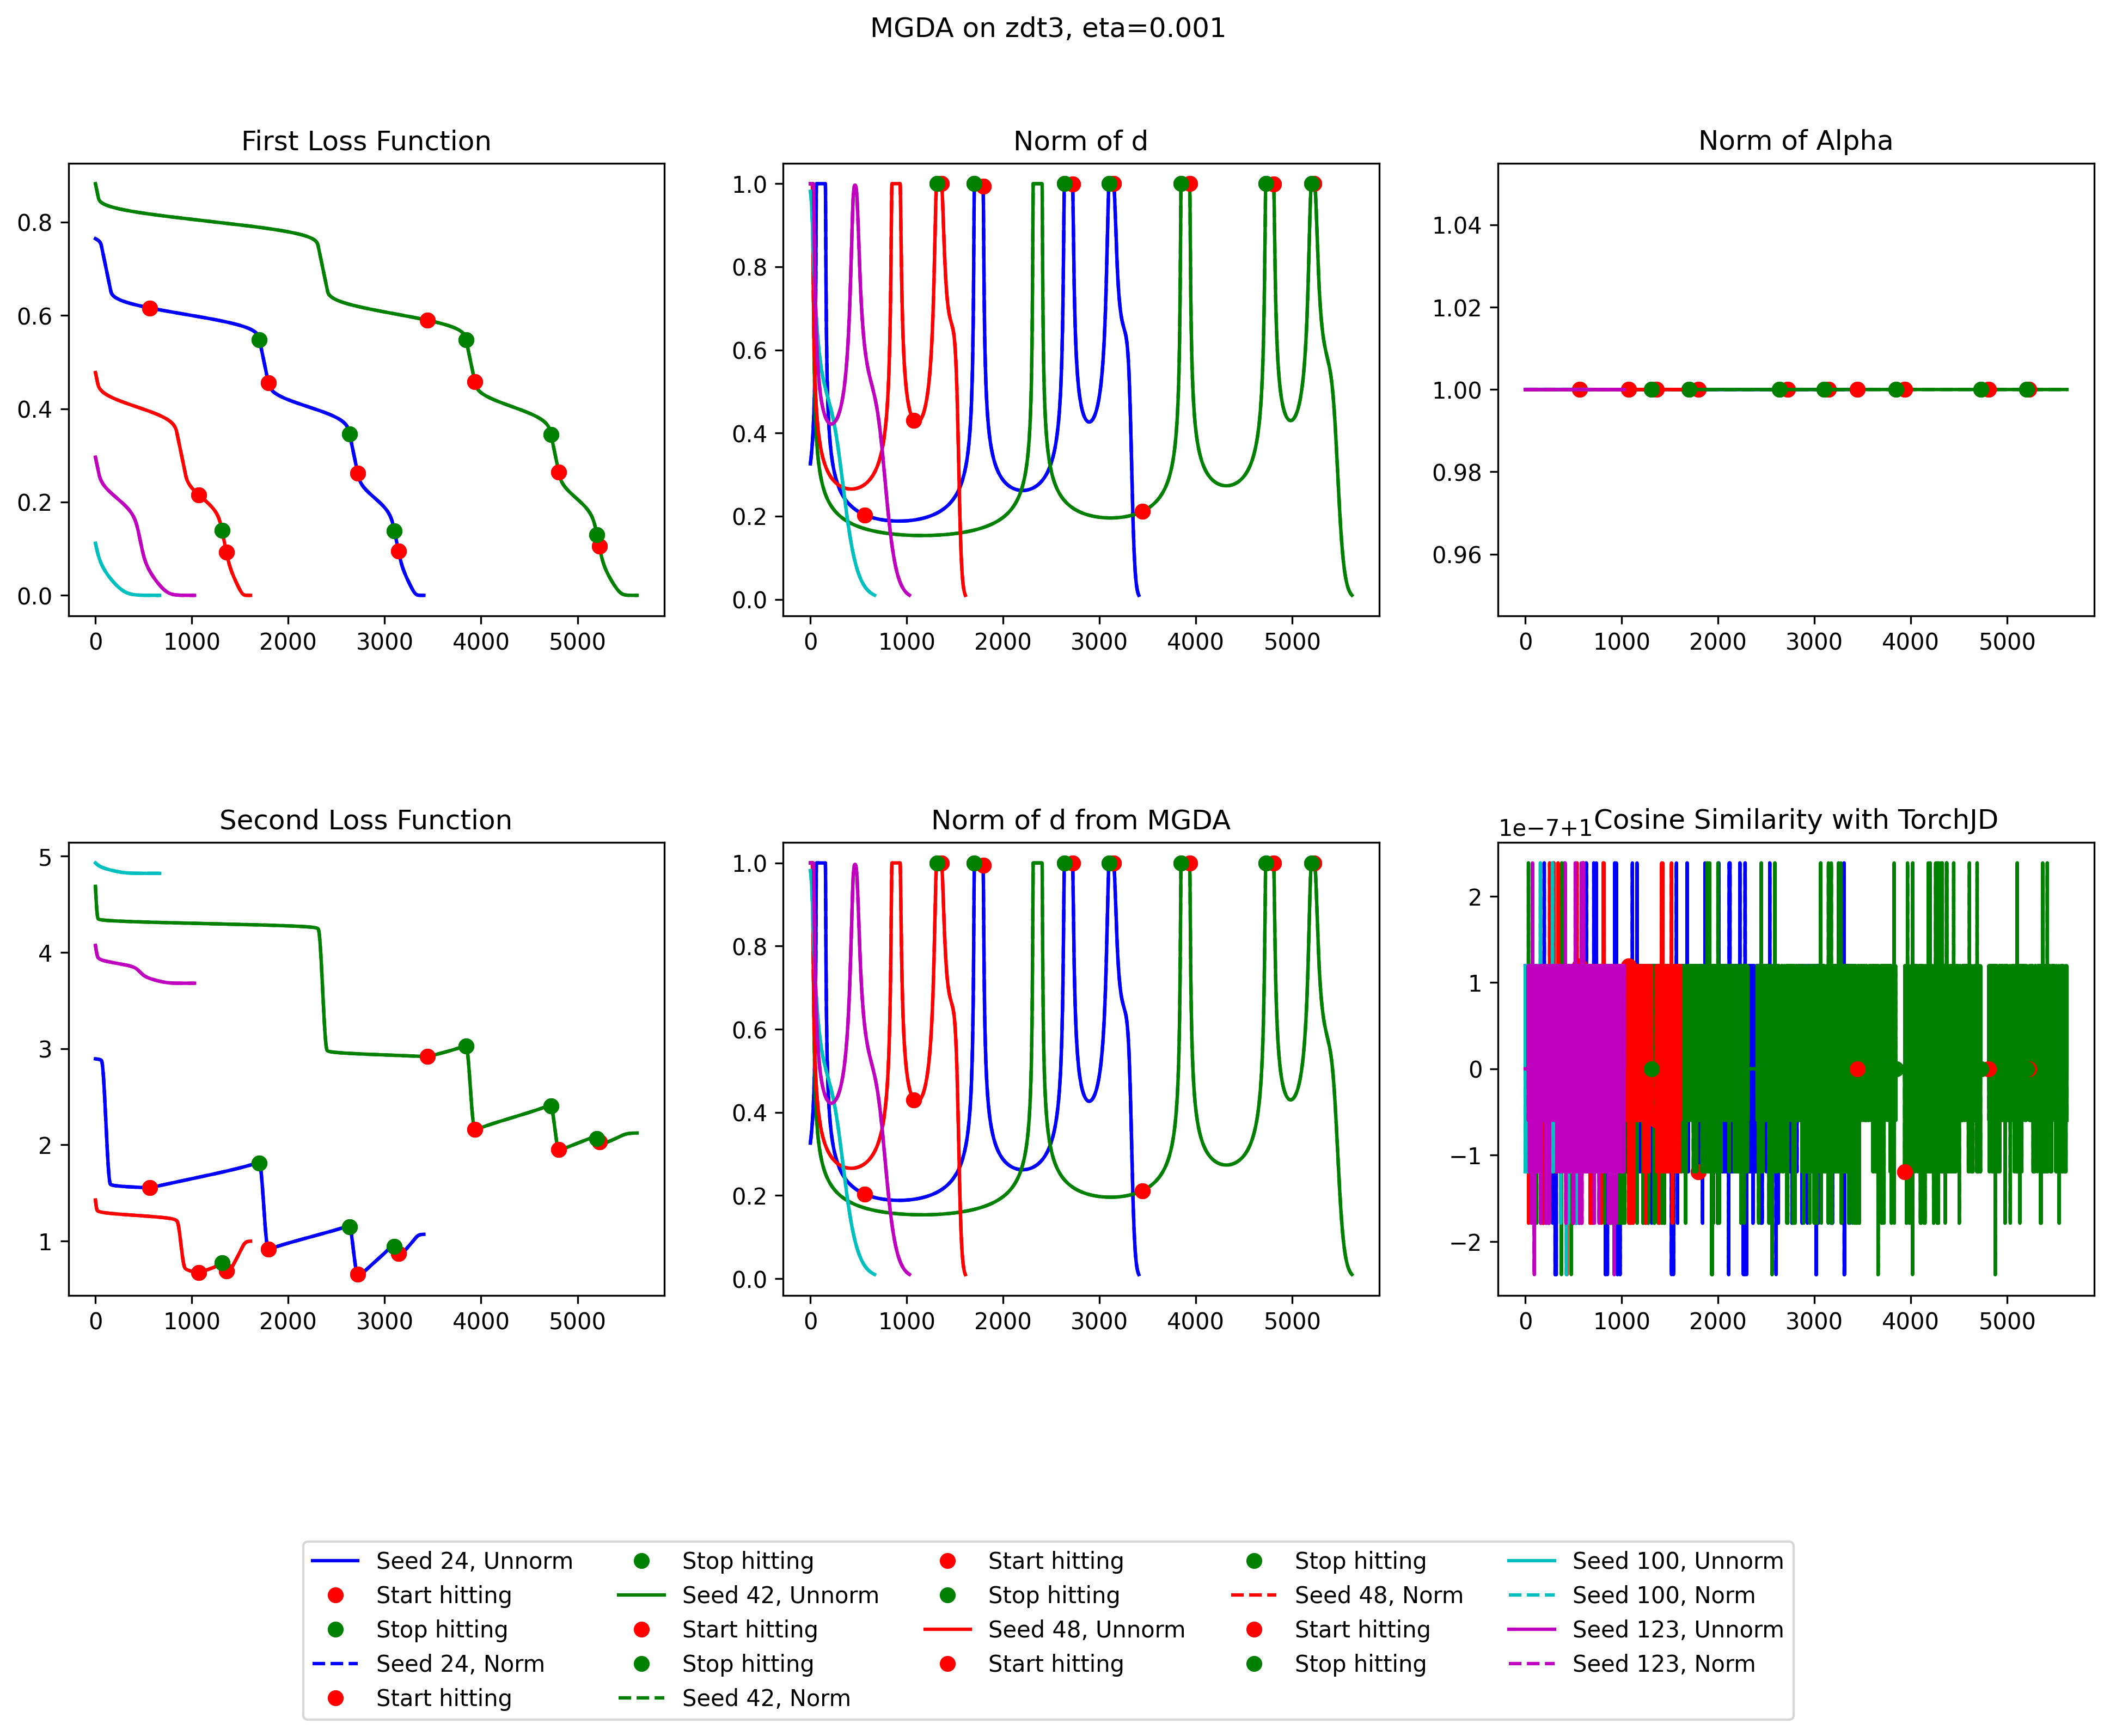
\includegraphics[scale=0.4]{MGDA_zdt3.png}
            \caption{Testing MGDA on ZDT3, with dimension = 4, learning rate = 0.001, max iteration = 10000, seed = 24, 42, 48, 100, 123. The red dots indicate the points where the sequence $x_t$ hit the boundary of the feasible region. And green dots indicate when the sequence leaves the boundary and reenters the interior of the feasible region.}
        \end{figure}
        \begin{figure}[h]
            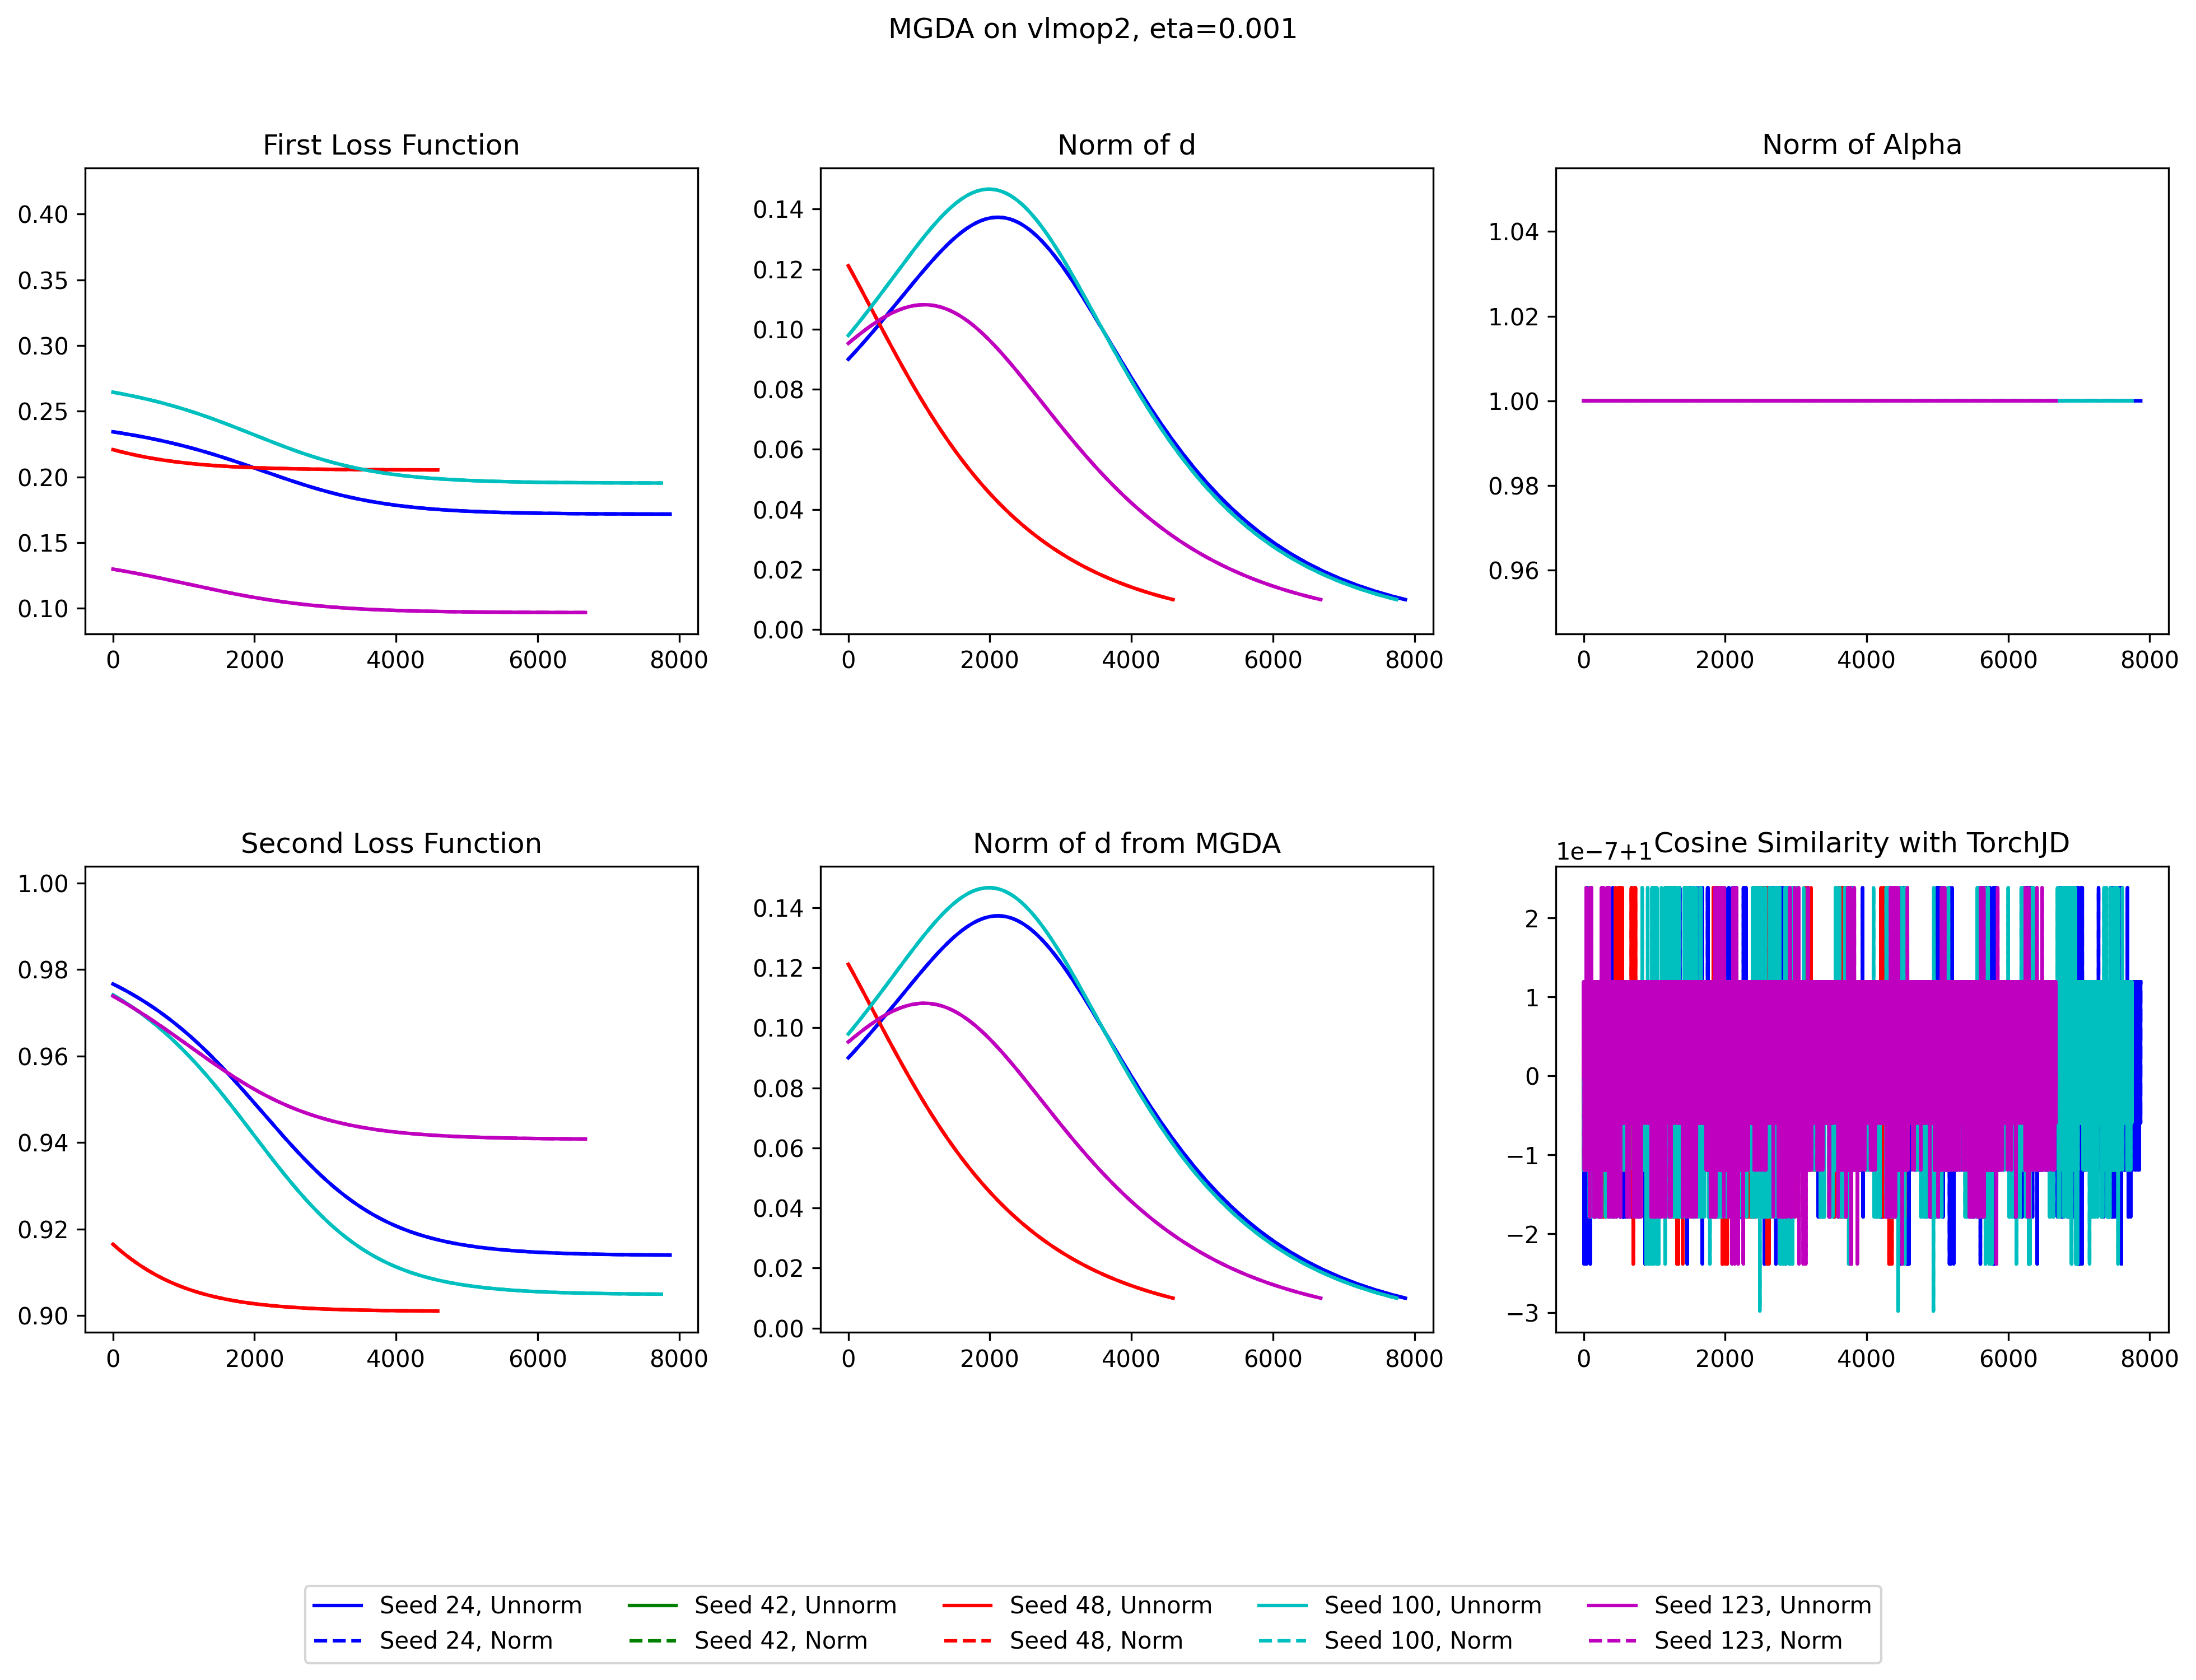
\includegraphics[scale=0.4]{MGDA_vlmop2.png}
            \caption{Testing MGDA on VLMOP2, with dimension = 4, learning rate = 0.001, max iteration = 10000, seed = 24, 42, 48, 100, 123.}
        \end{figure}
        \begin{figure}[h]
            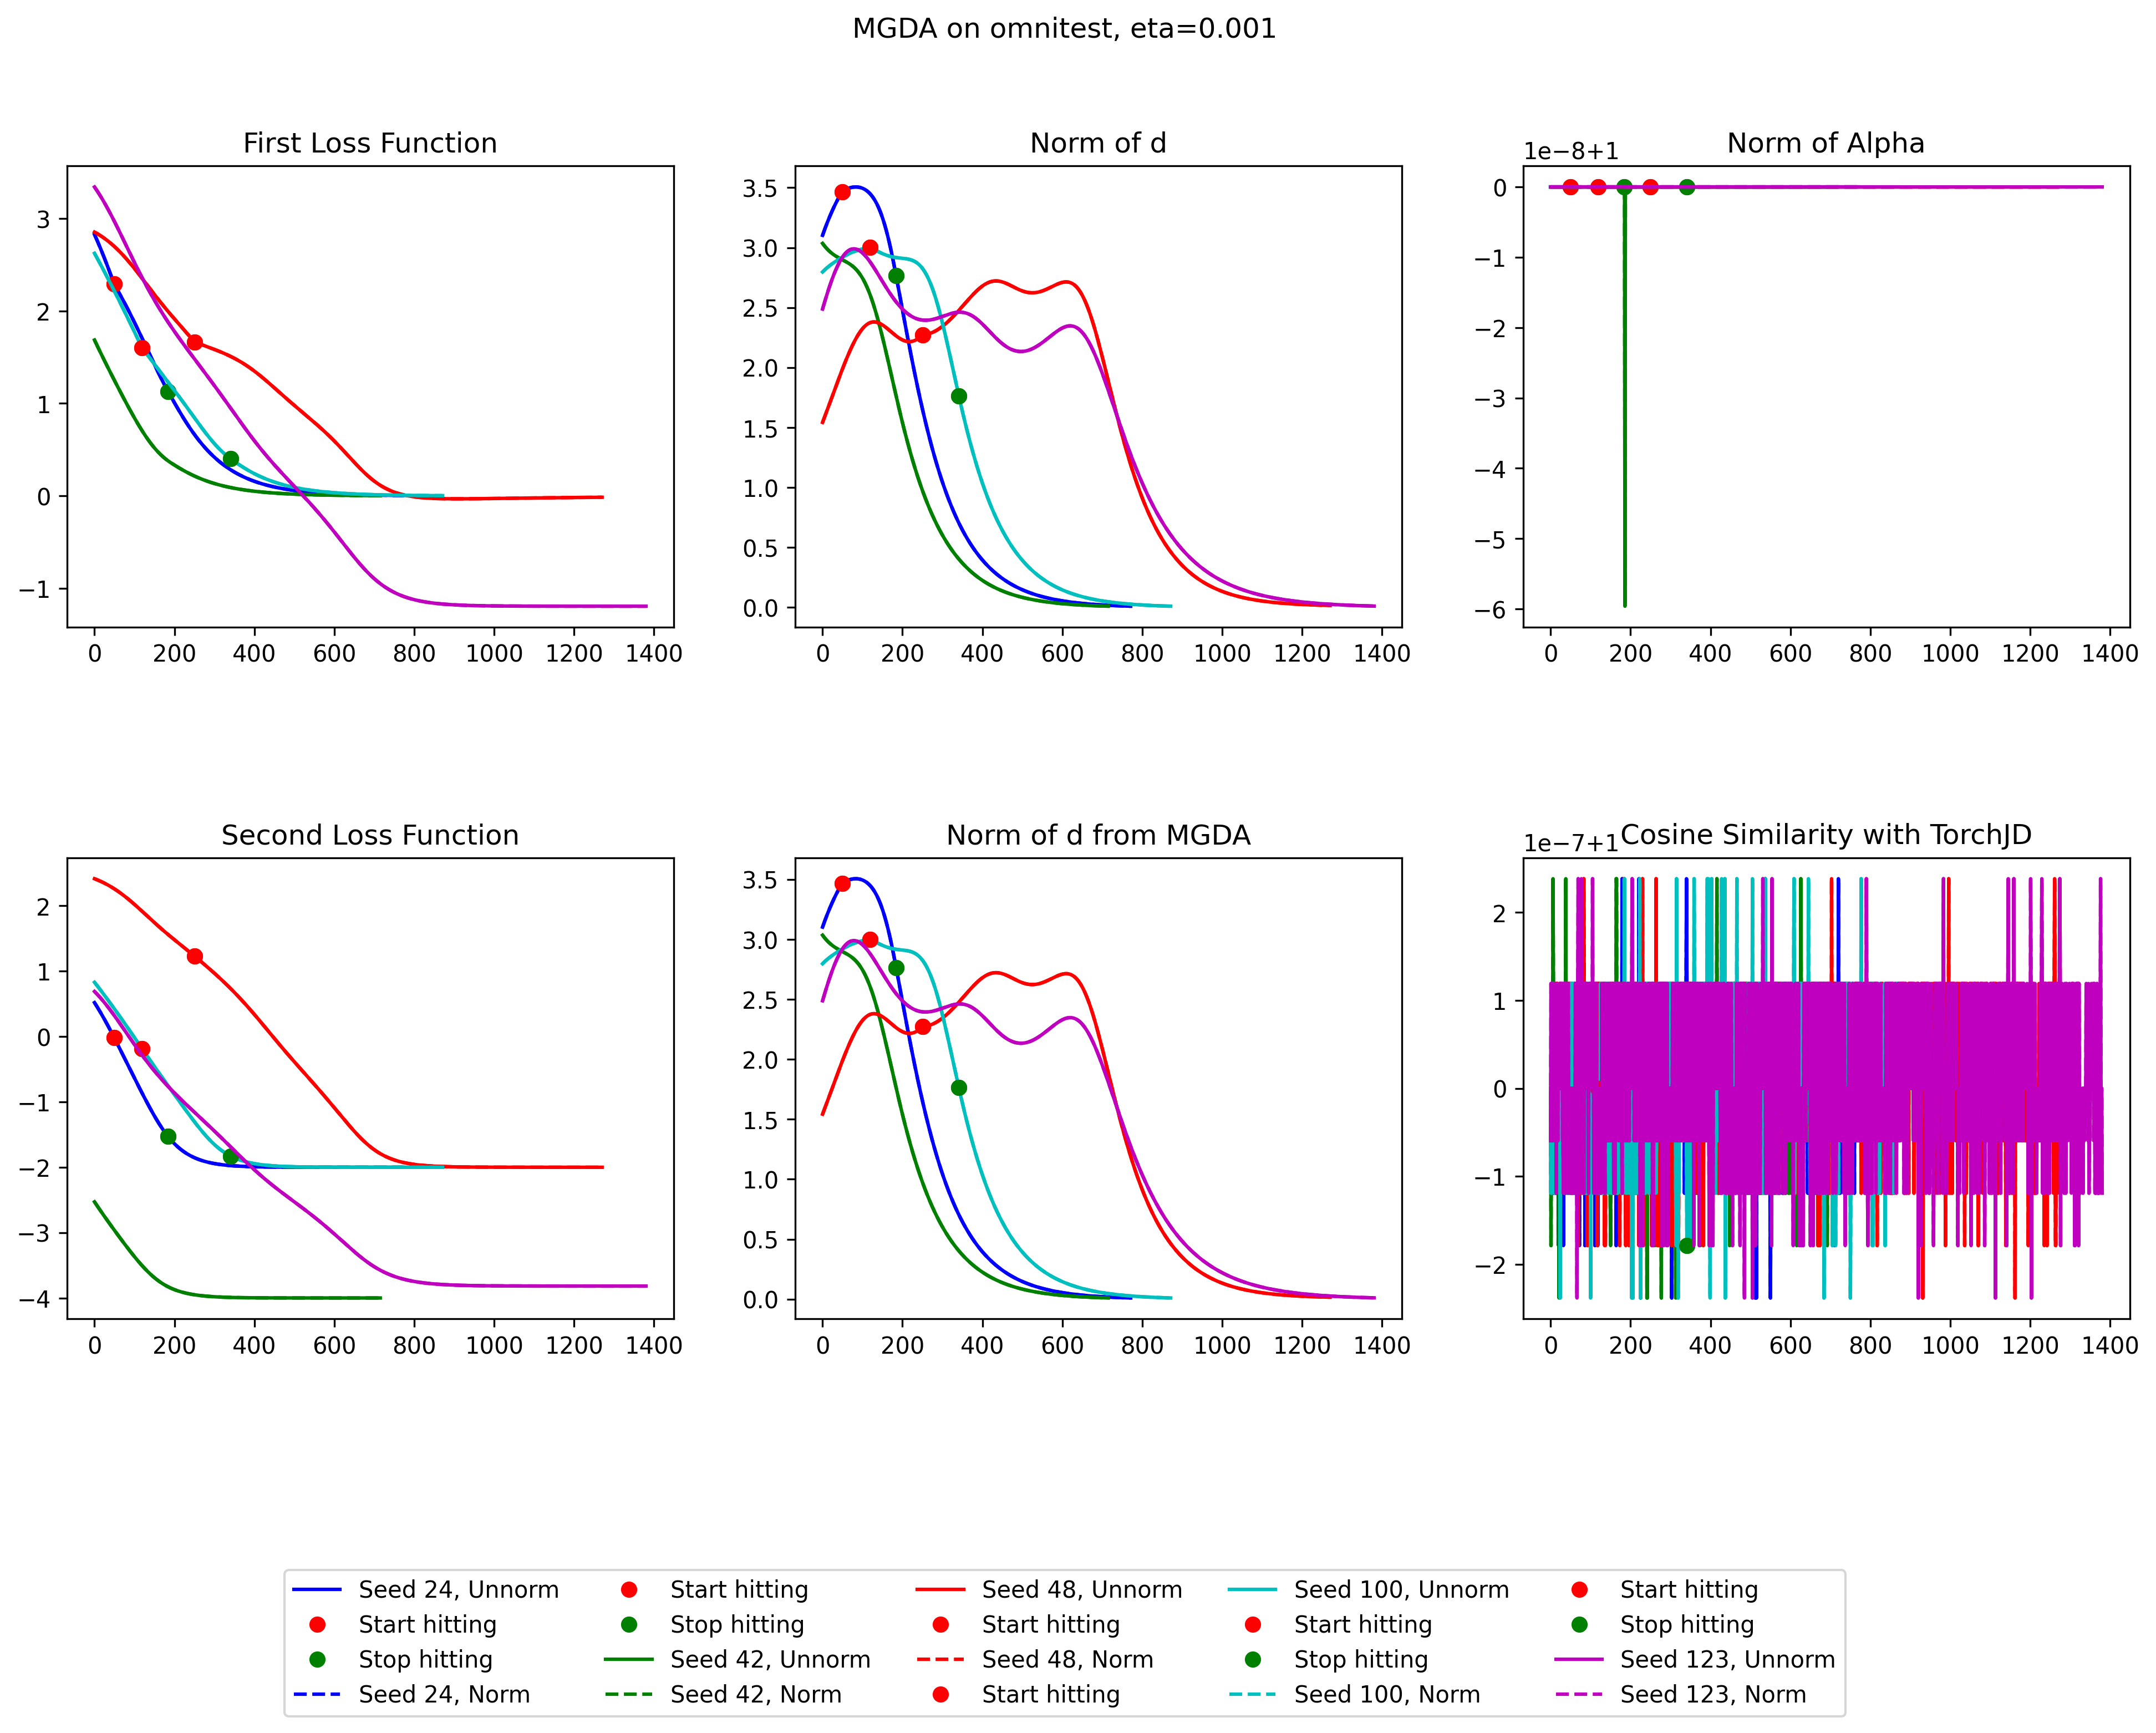
\includegraphics[scale=0.4]{MGDA_omnitest.png}
            \caption{Testing MGDA on Omniset, with dimension = 4, learning rate = 0.001, max iteration = 10000, seed = 24, 42, 48, 100, 123. The red dots indicate the points where the sequence $x_t$ hit the boundary of the feasible region. And green dots indicate when the sequence leaves the boundary and reenters the interior of the feasible region.}
        \end{figure}
    \end{center}
    \section{DualProj and UPGrad}
    Since the behaviour of DualProj and UPGrad are similar, we will group them into the same section.\\
    In general, the two aggregators performed fairly well in VLMOP2, as the descent algorithm managed to converge to Pareto Stationarity under both aggreators for all seeds. Difficulties arises in Omnitest. In cases where the descent algorithm hits the boundary of the feasible region (random seed 24, 48, 100), the algorithm converge to a non-Pareto stationary point at the boundary. Though in cases where the algorithm does not reach the boundary, it always converge to Pareto stationary. However, ZDT3 is extremely difficult for both aggregators. The descent algorithms hit the boundary in all cases and converges to a non-Pareto stationary point at the boundary.\\
    Comparing across different synthetic problems, we observe that with normalisation, the algorithm tend to converge slower than without normalisation, though the normalised and unnormalised version of the descent algorithm always converge to the same point. As a result of slower convergence, sudden jumps in the course of iteration could be smoothed out. For example, when UPGrad is tested on ZDT3 with random seed 123, a sudden jump in the norm of $d$ can be seen if no normalisation is applied. After applying normalisation, the sudden jump became a smooth peak. In general, the two aggregators is less robust than MGDA, but have better performance than Nash-MTL.
        \begin{center}
        \begin{figure}[h]
            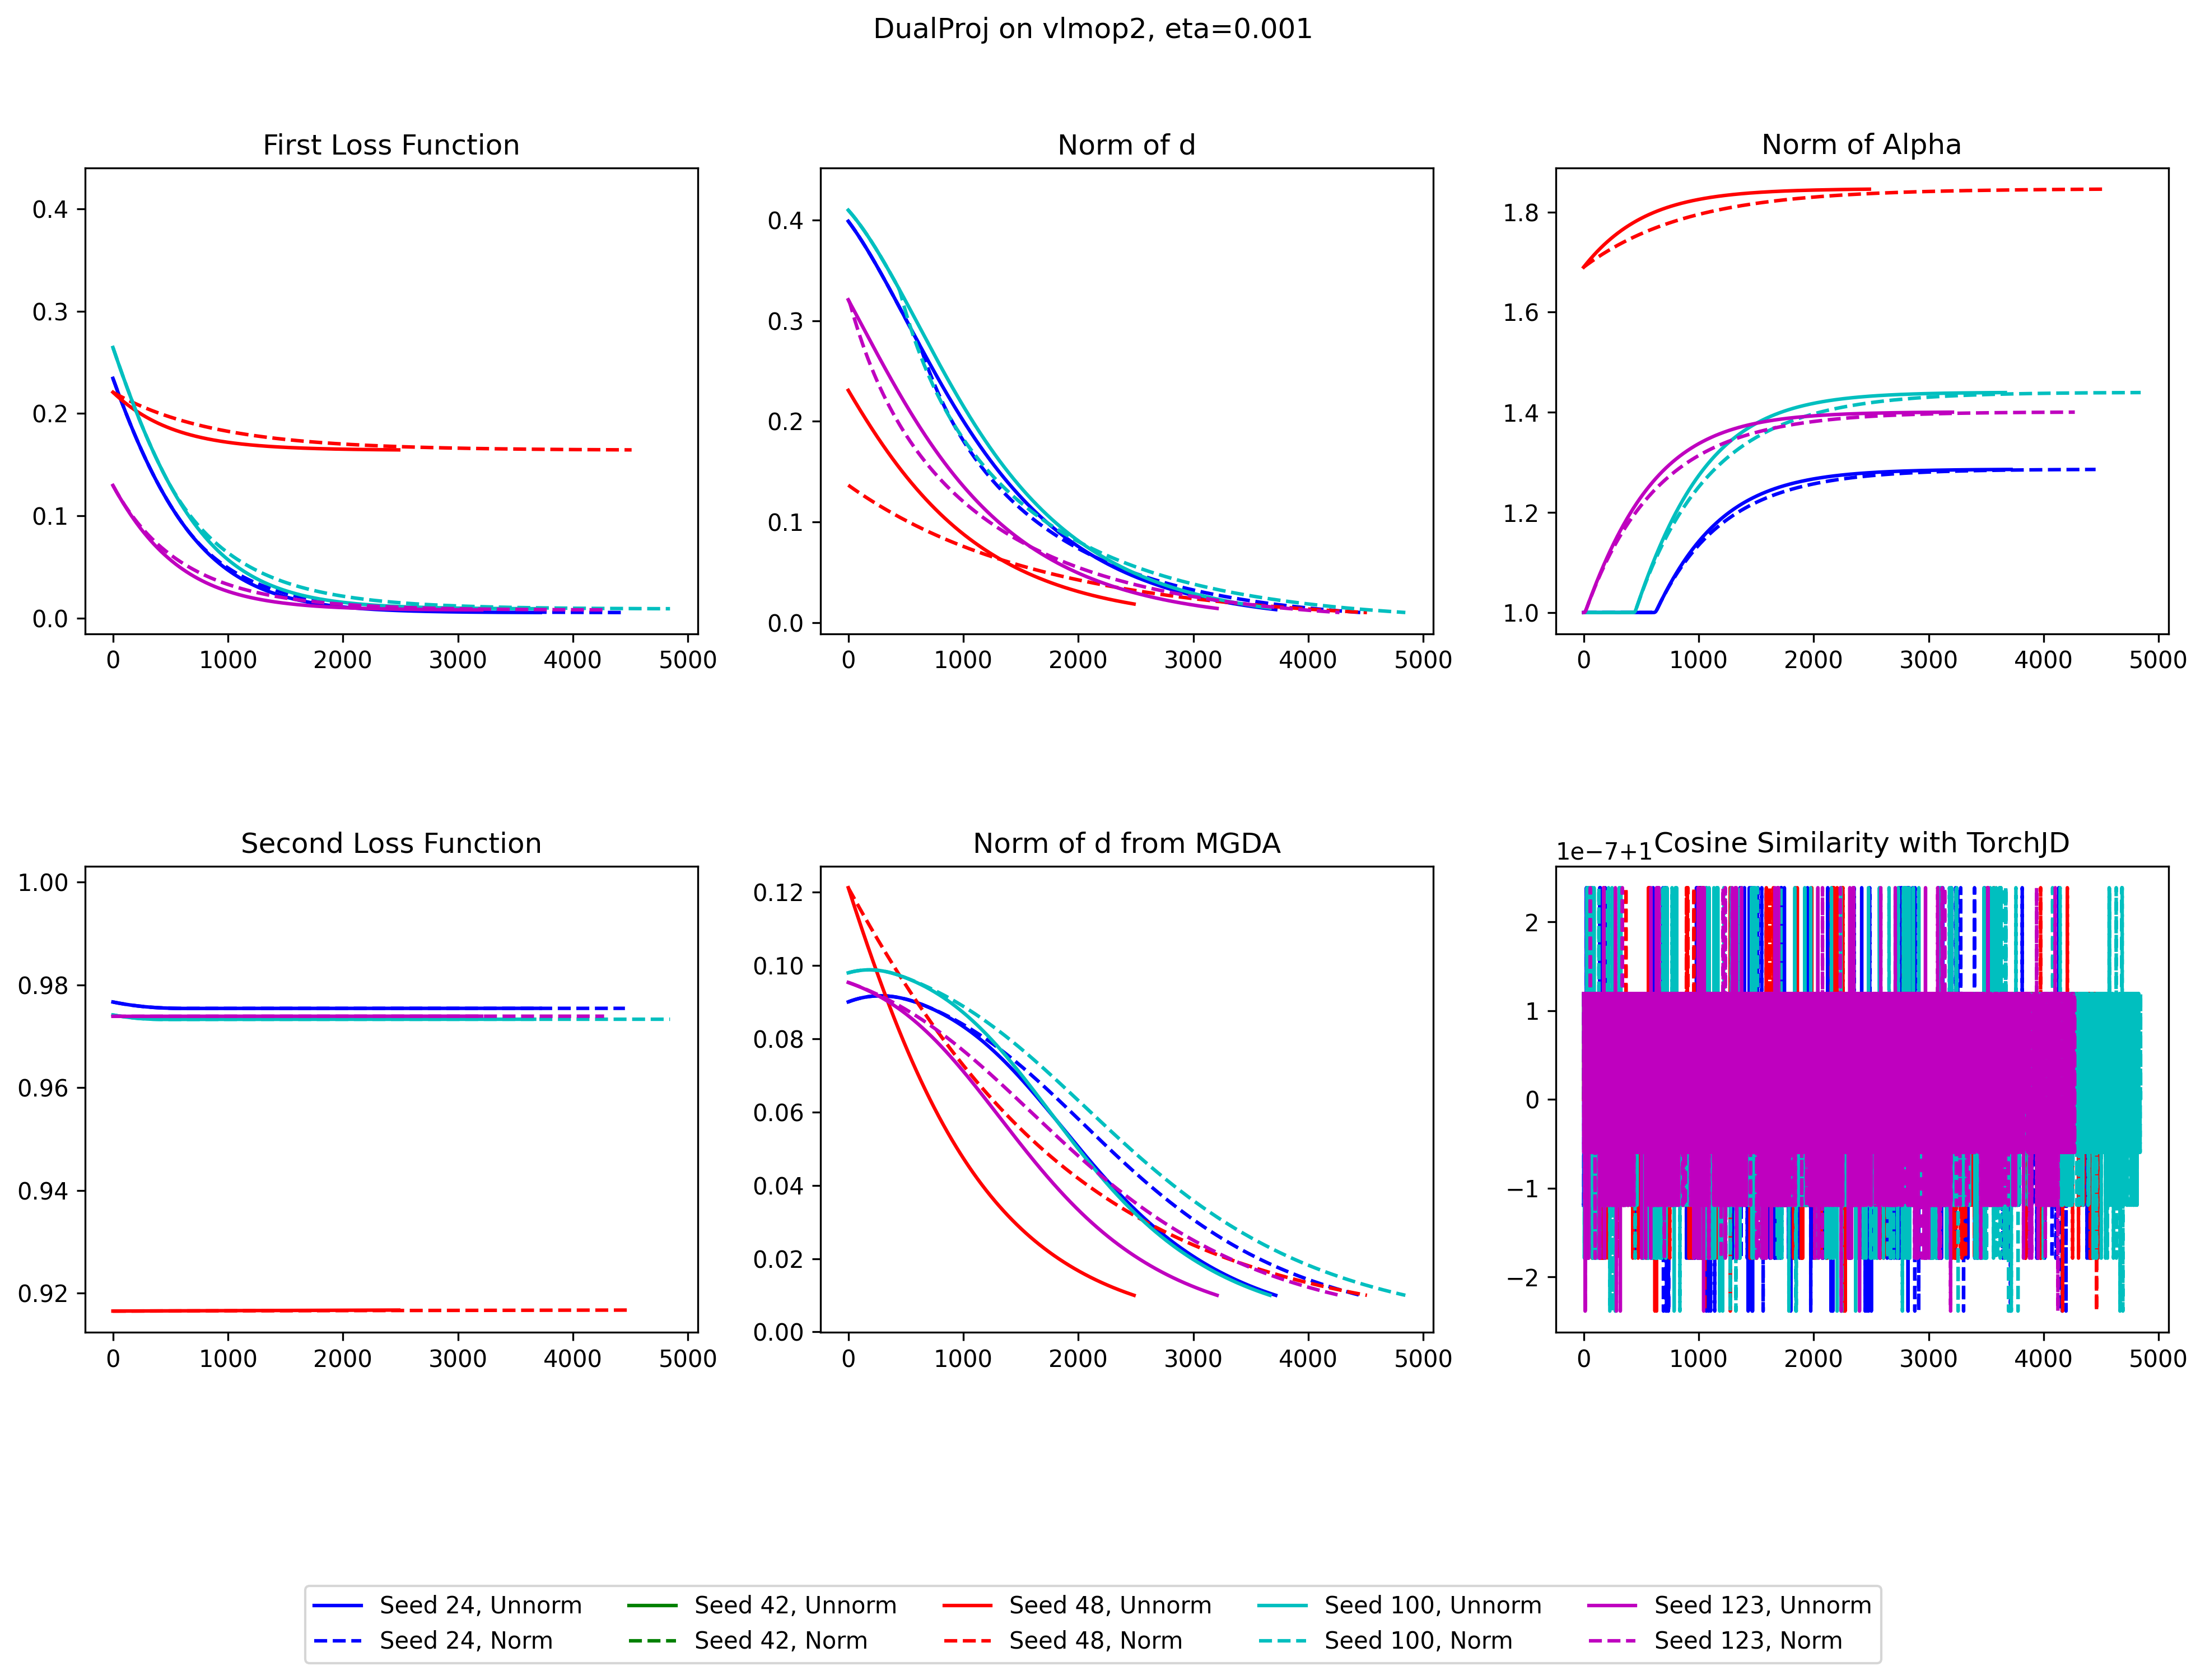
\includegraphics[scale=0.4]{DualProj_vlmop2.png}
            \caption{Testing DualProj on VLMOP2, dimension = 4, learning rate = 0.001, max iteration = 10000, seeds = 24, 42, 48, 100, 123.}
        \end{figure}
        \begin{figure}[h]
            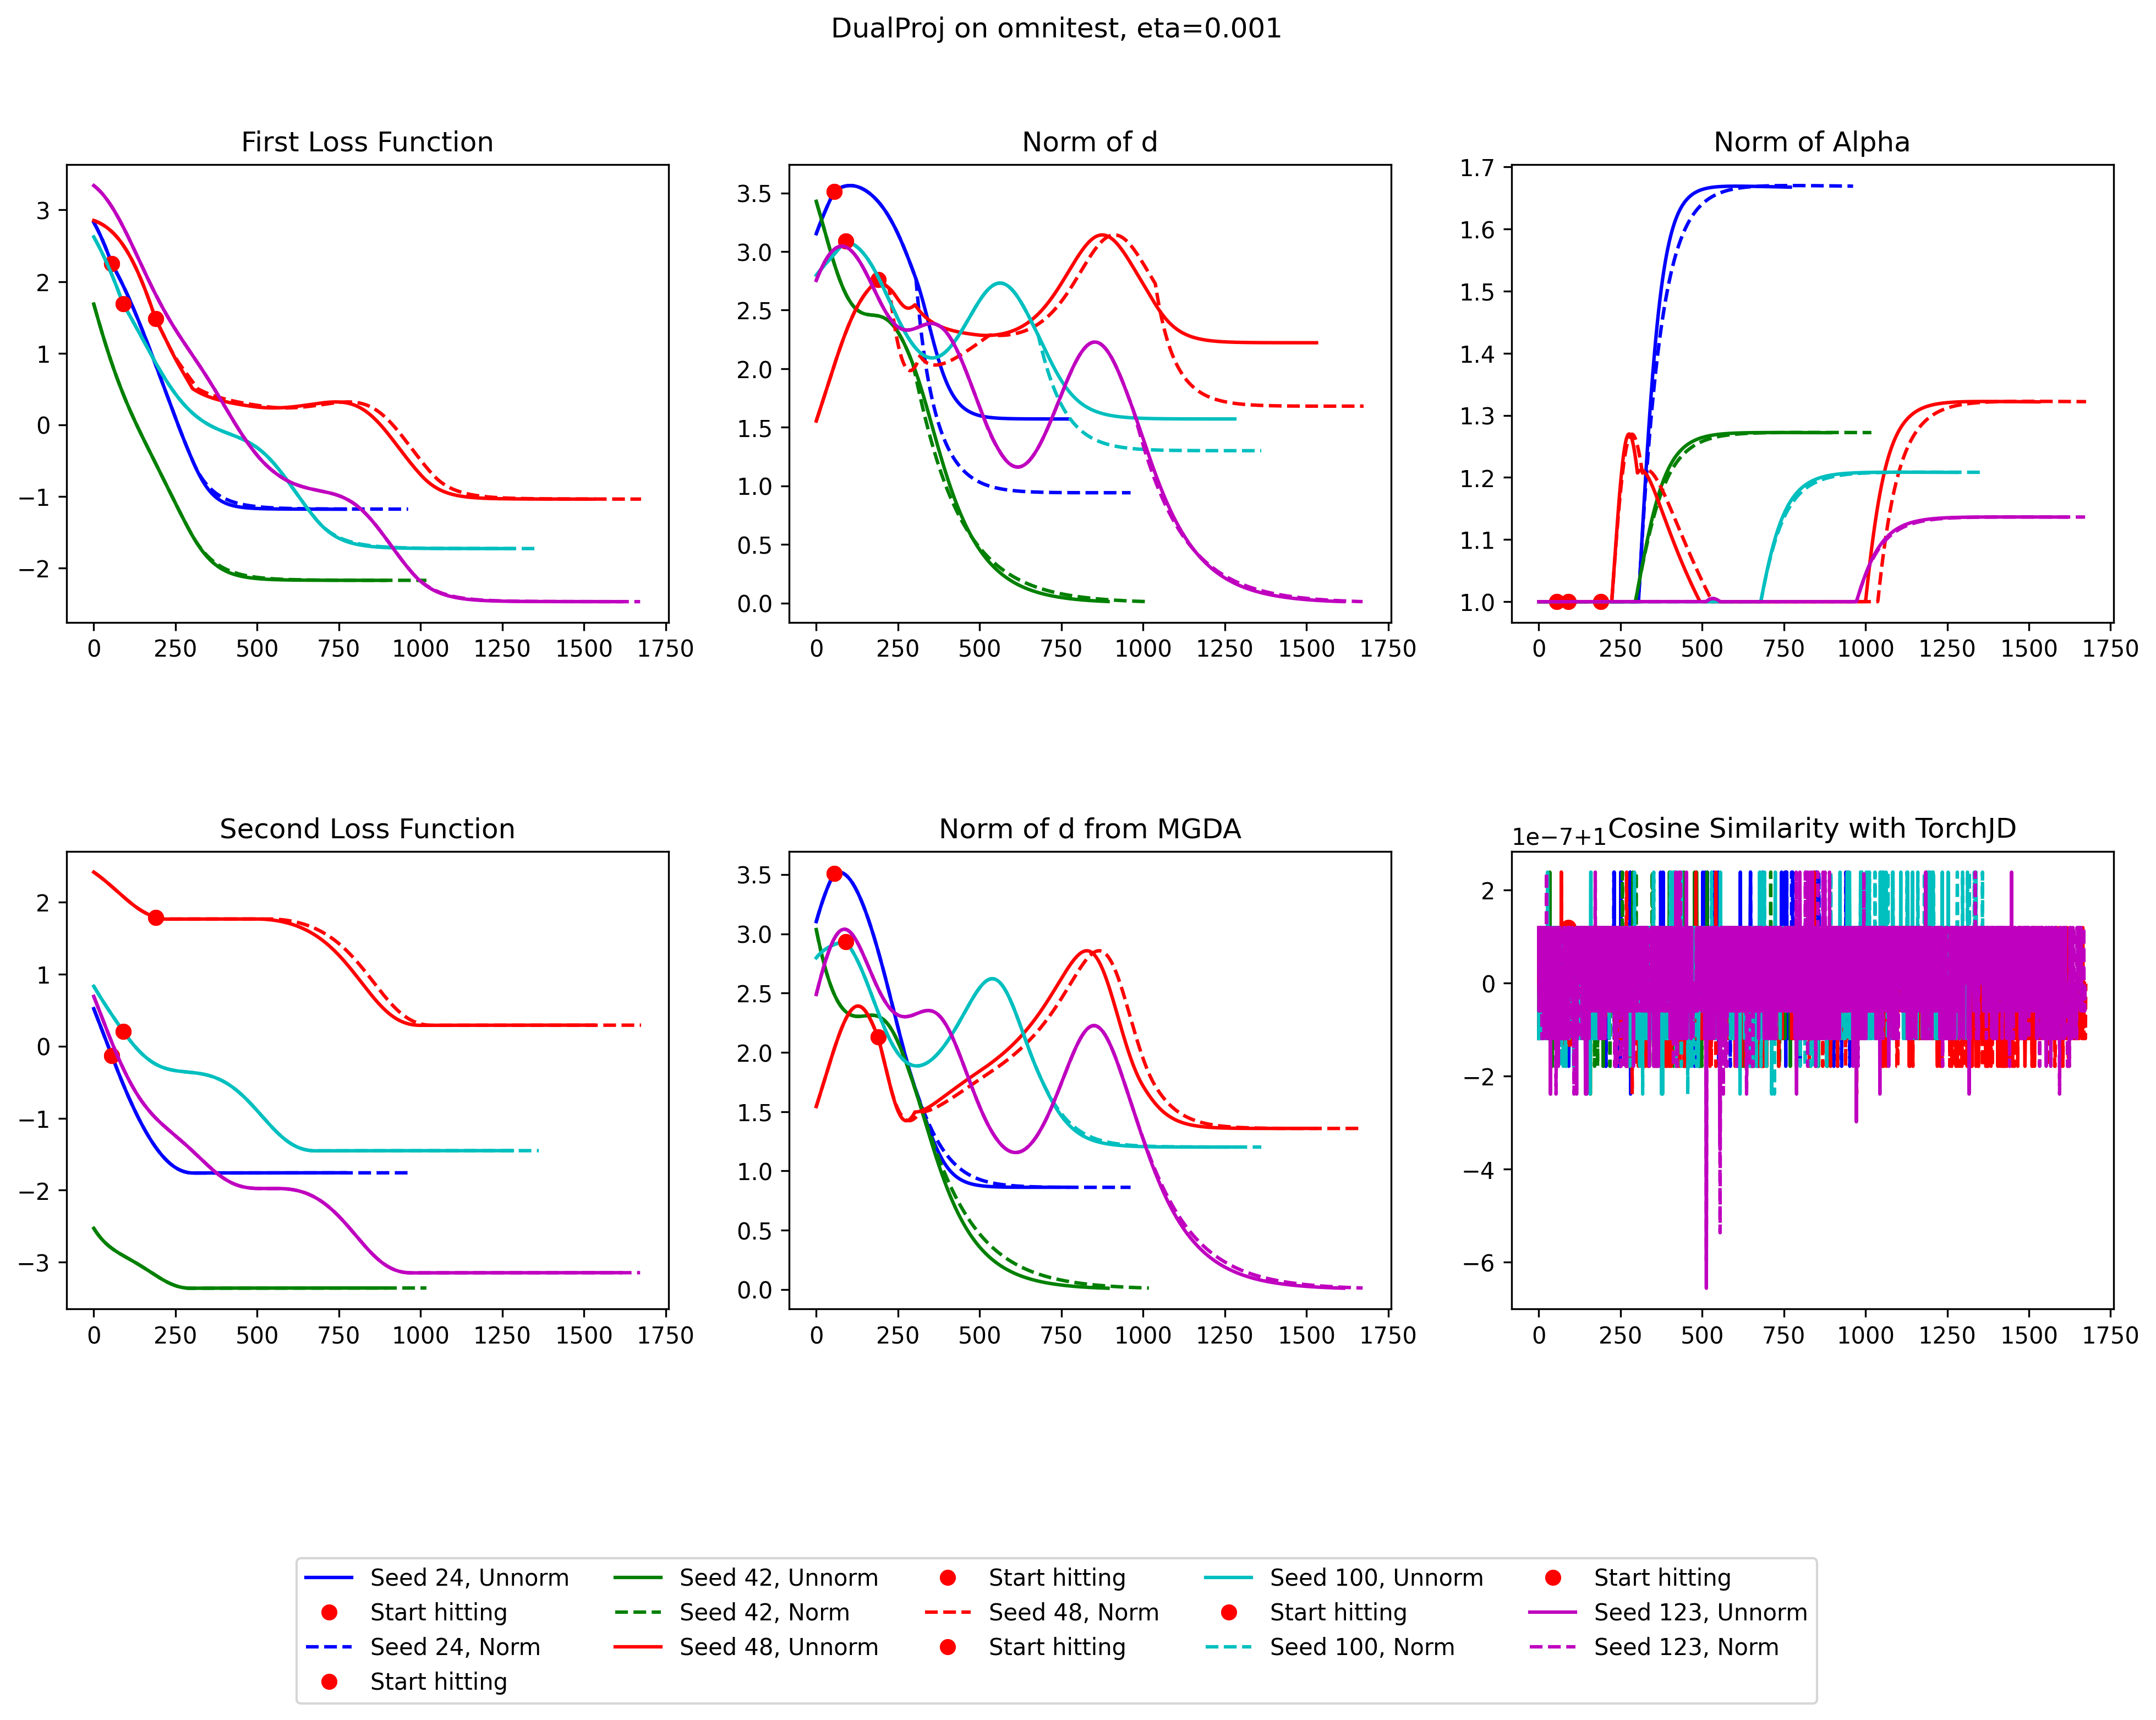
\includegraphics[scale=0.4]{DualProj_omnitest.png}
            \caption{Testing DualProj on Omnitest, dimension = 4, learning rate = 0.001, max iteration = 10000, seeds = 24, 42, 48, 100, 123. Red dots: $x_t$ hits boundary; green dots: $x_t$ reenters interior.}
        \end{figure}
        \begin{figure}[h]
            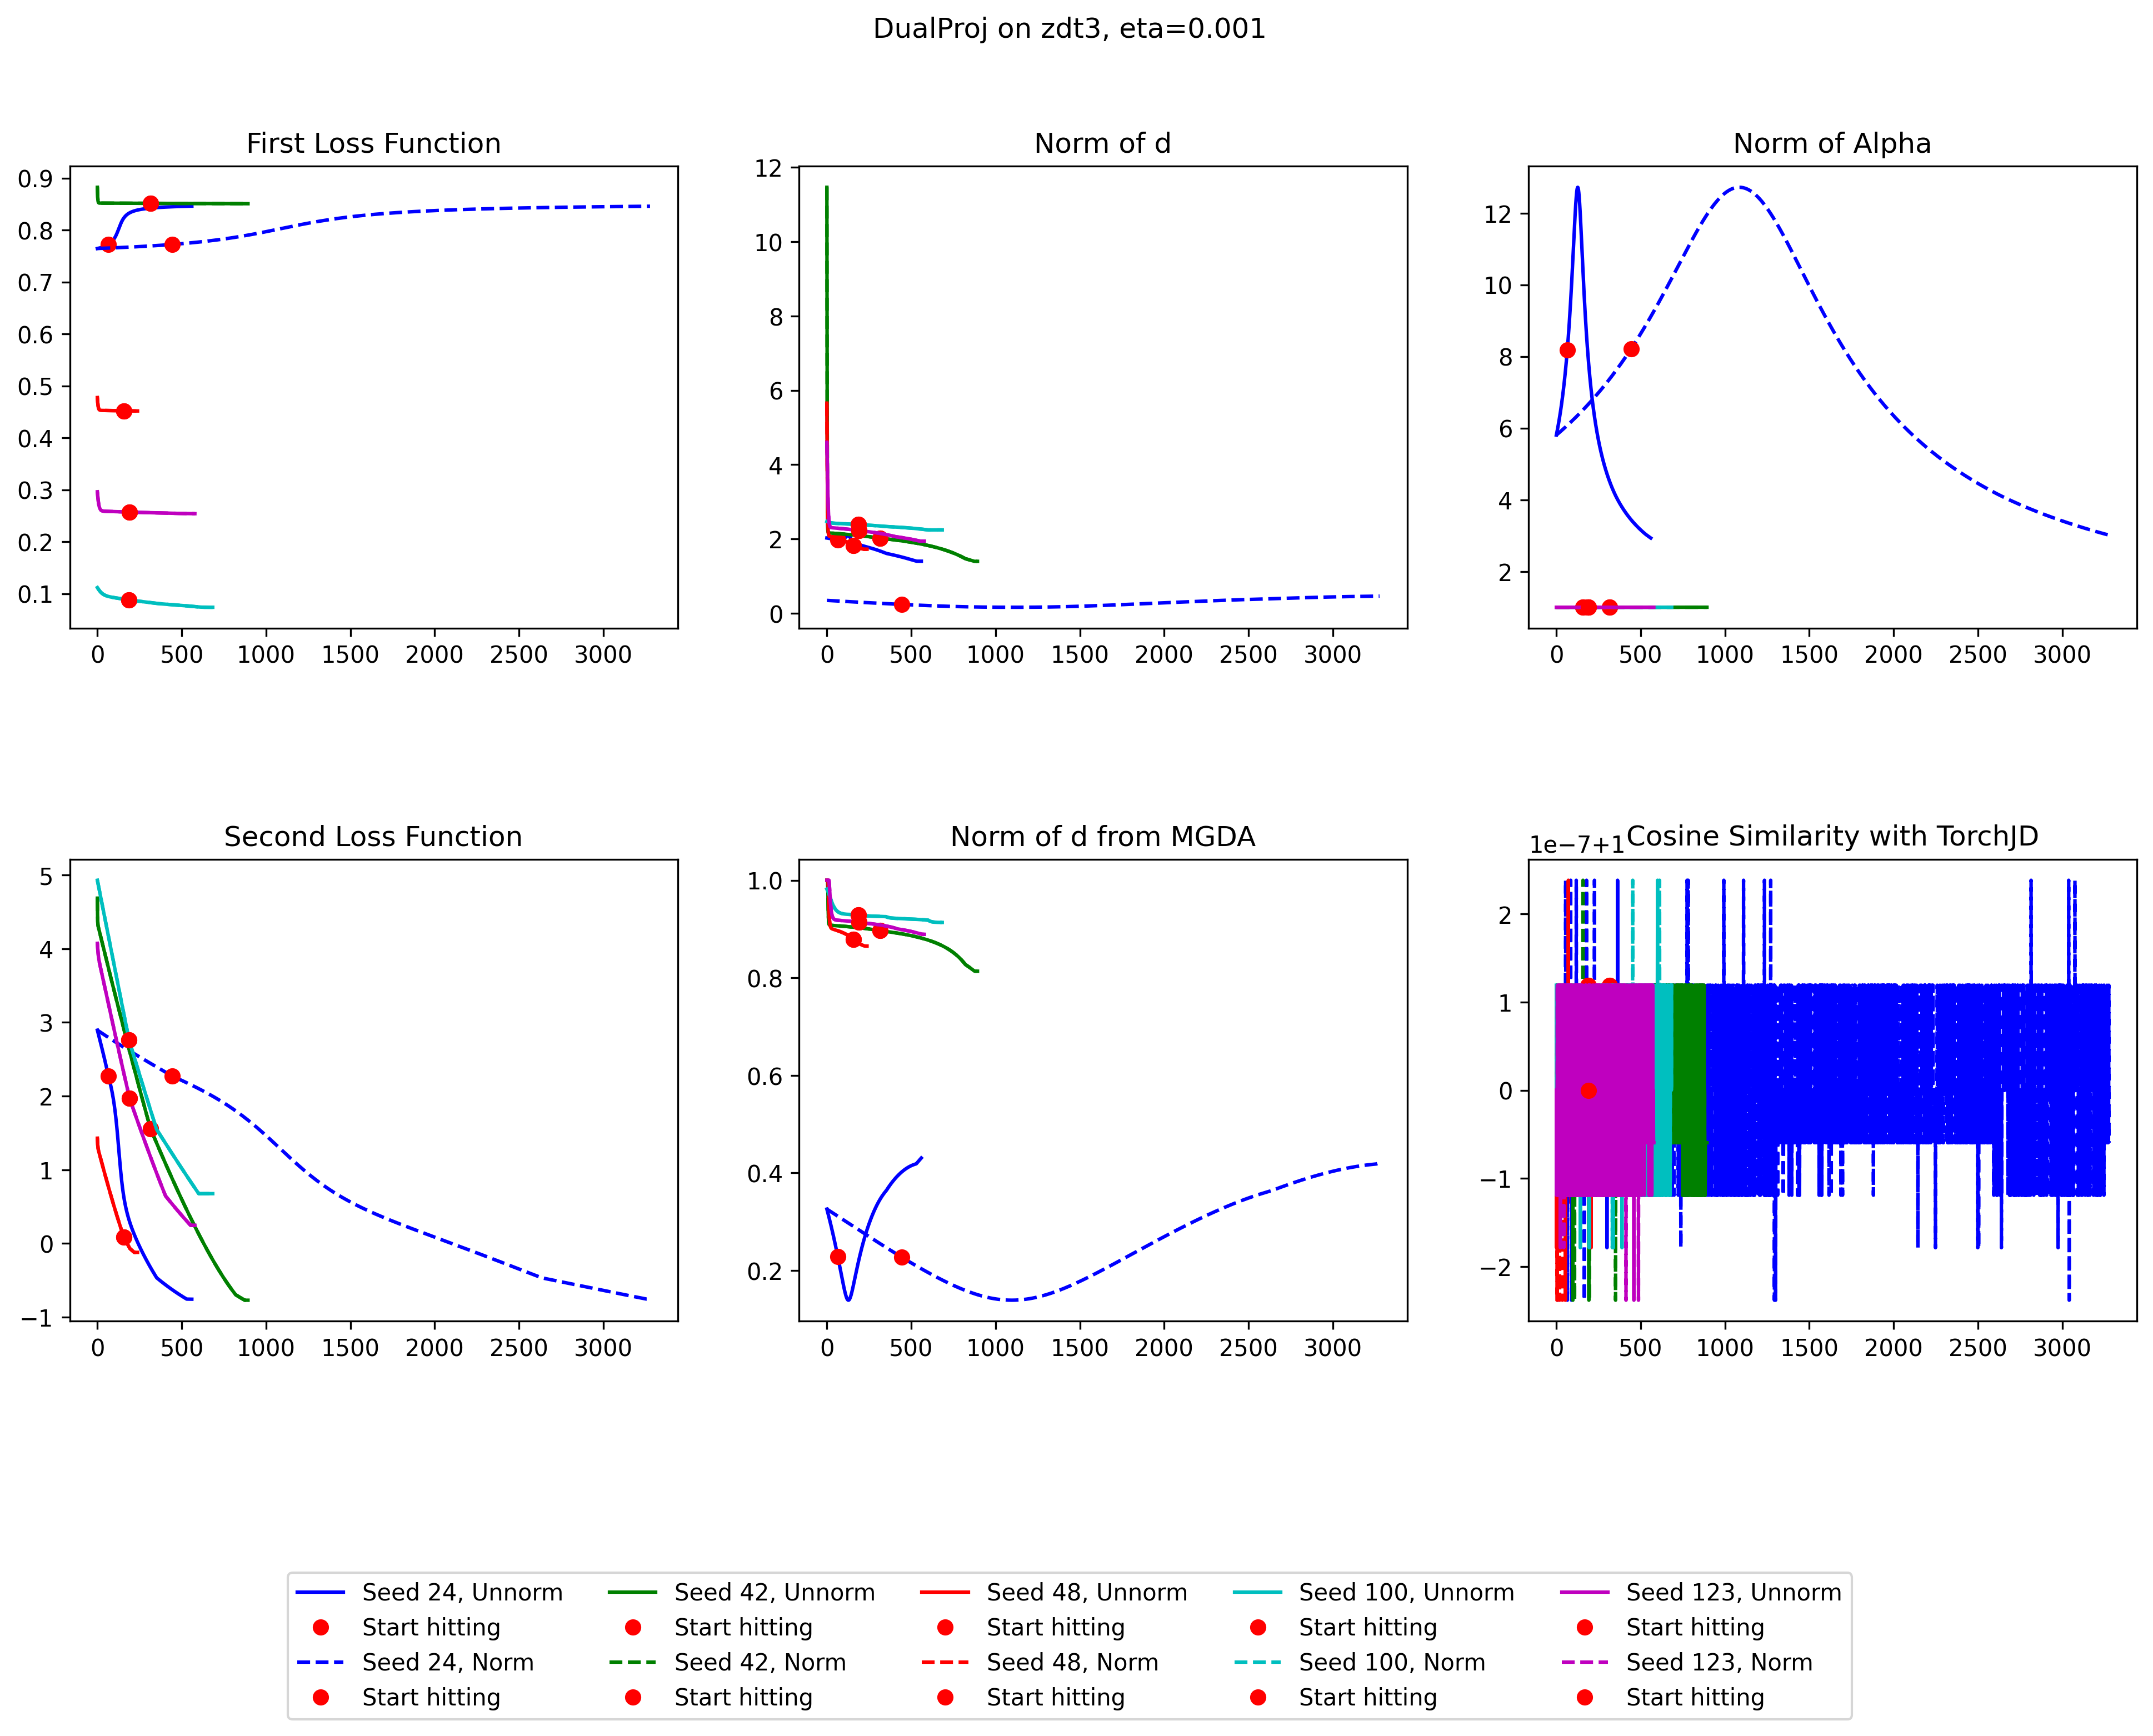
\includegraphics[scale=0.4]{DualProj_zdt3.png}
            \caption{Testing DualProj on ZDT3, dimension = 4, learning rate = 0.001, max iteration = 10000, seeds = 24, 42, 48, 100, 123. Red dots: $x_t$ hits boundary; green dots: $x_t$ reenters interior.}
        \end{figure}
        \begin{figure}[h]
            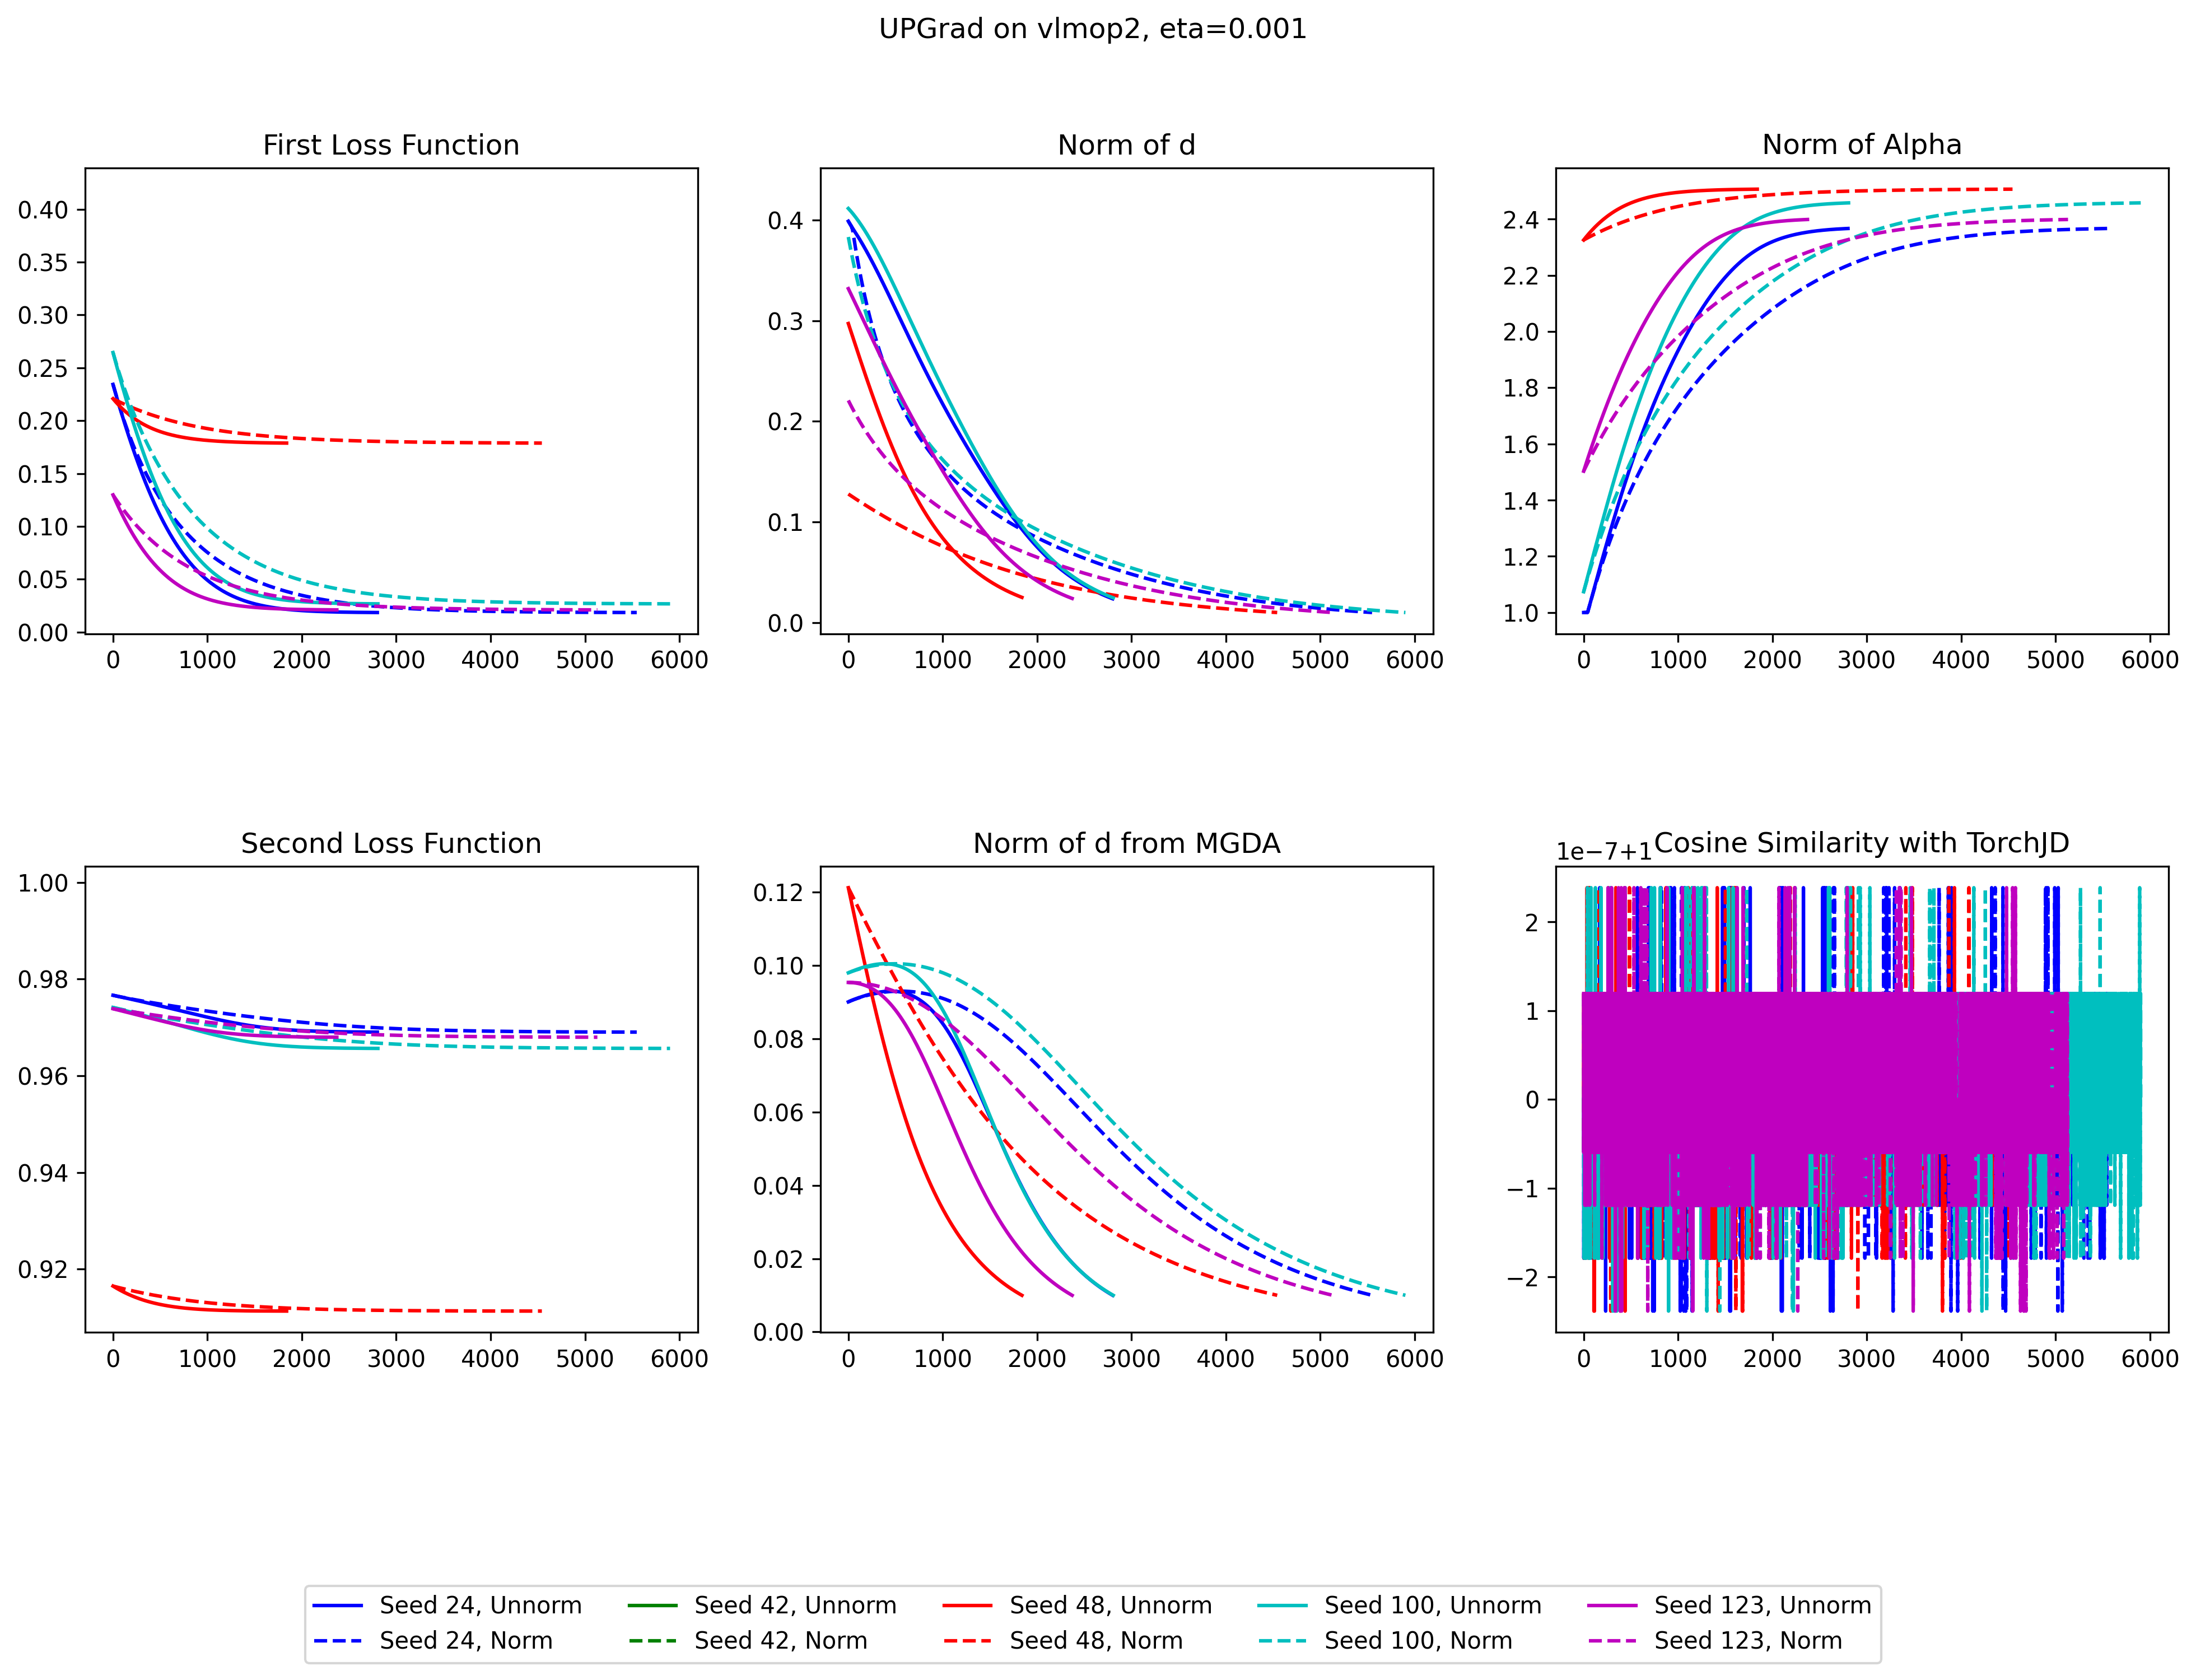
\includegraphics[scale=0.4]{UPGrad_vlmop2.png}
            \caption{Testing UPGrad on VLMOP2, dimension = 4, learning rate = 0.001, max iteration = 10000, seeds = 24, 42, 48, 100, 123.}
        \end{figure}
        \begin{figure}[h]
            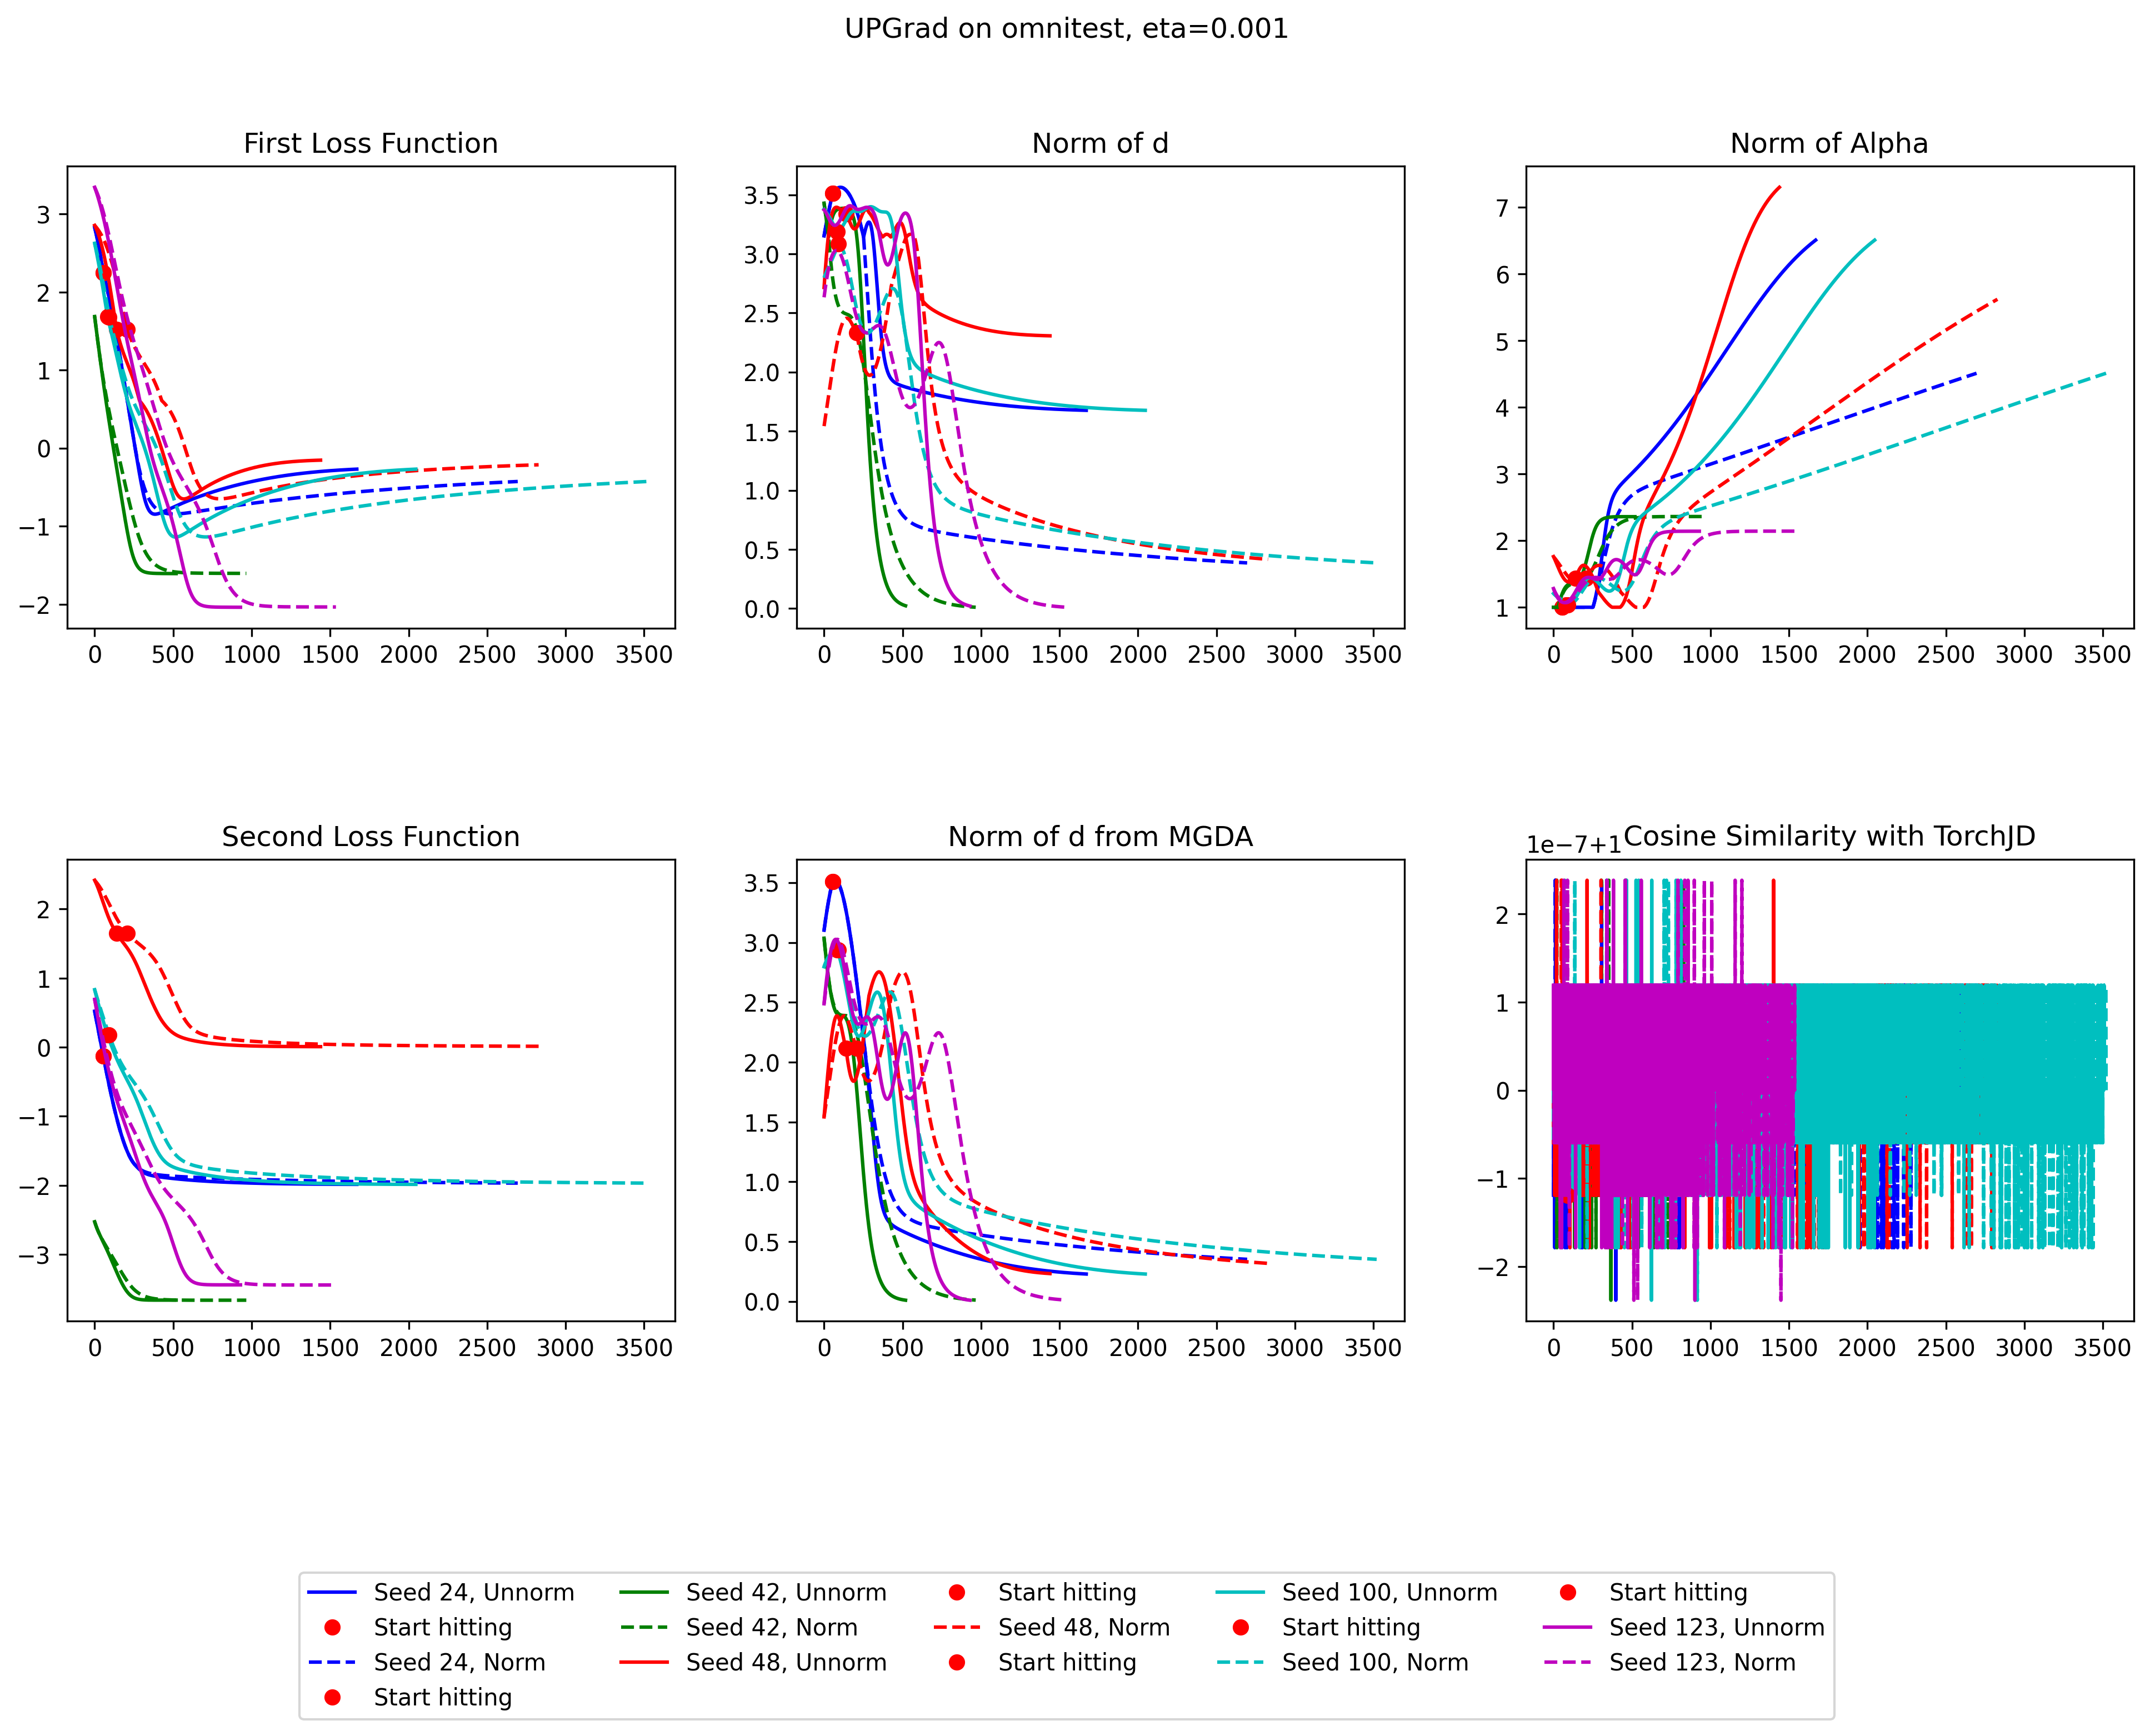
\includegraphics[scale=0.4]{UPGrad_omnitest.png}
            \caption{Testing UPGrad on Omnitest, dimension = 4, learning rate = 0.001, max iteration = 10000, seeds = 24, 42, 48, 100, 123. Red dots: $x_t$ hits boundary; green dots: $x_t$ reenters interior.}
        \end{figure}
        \begin{figure}[h]
            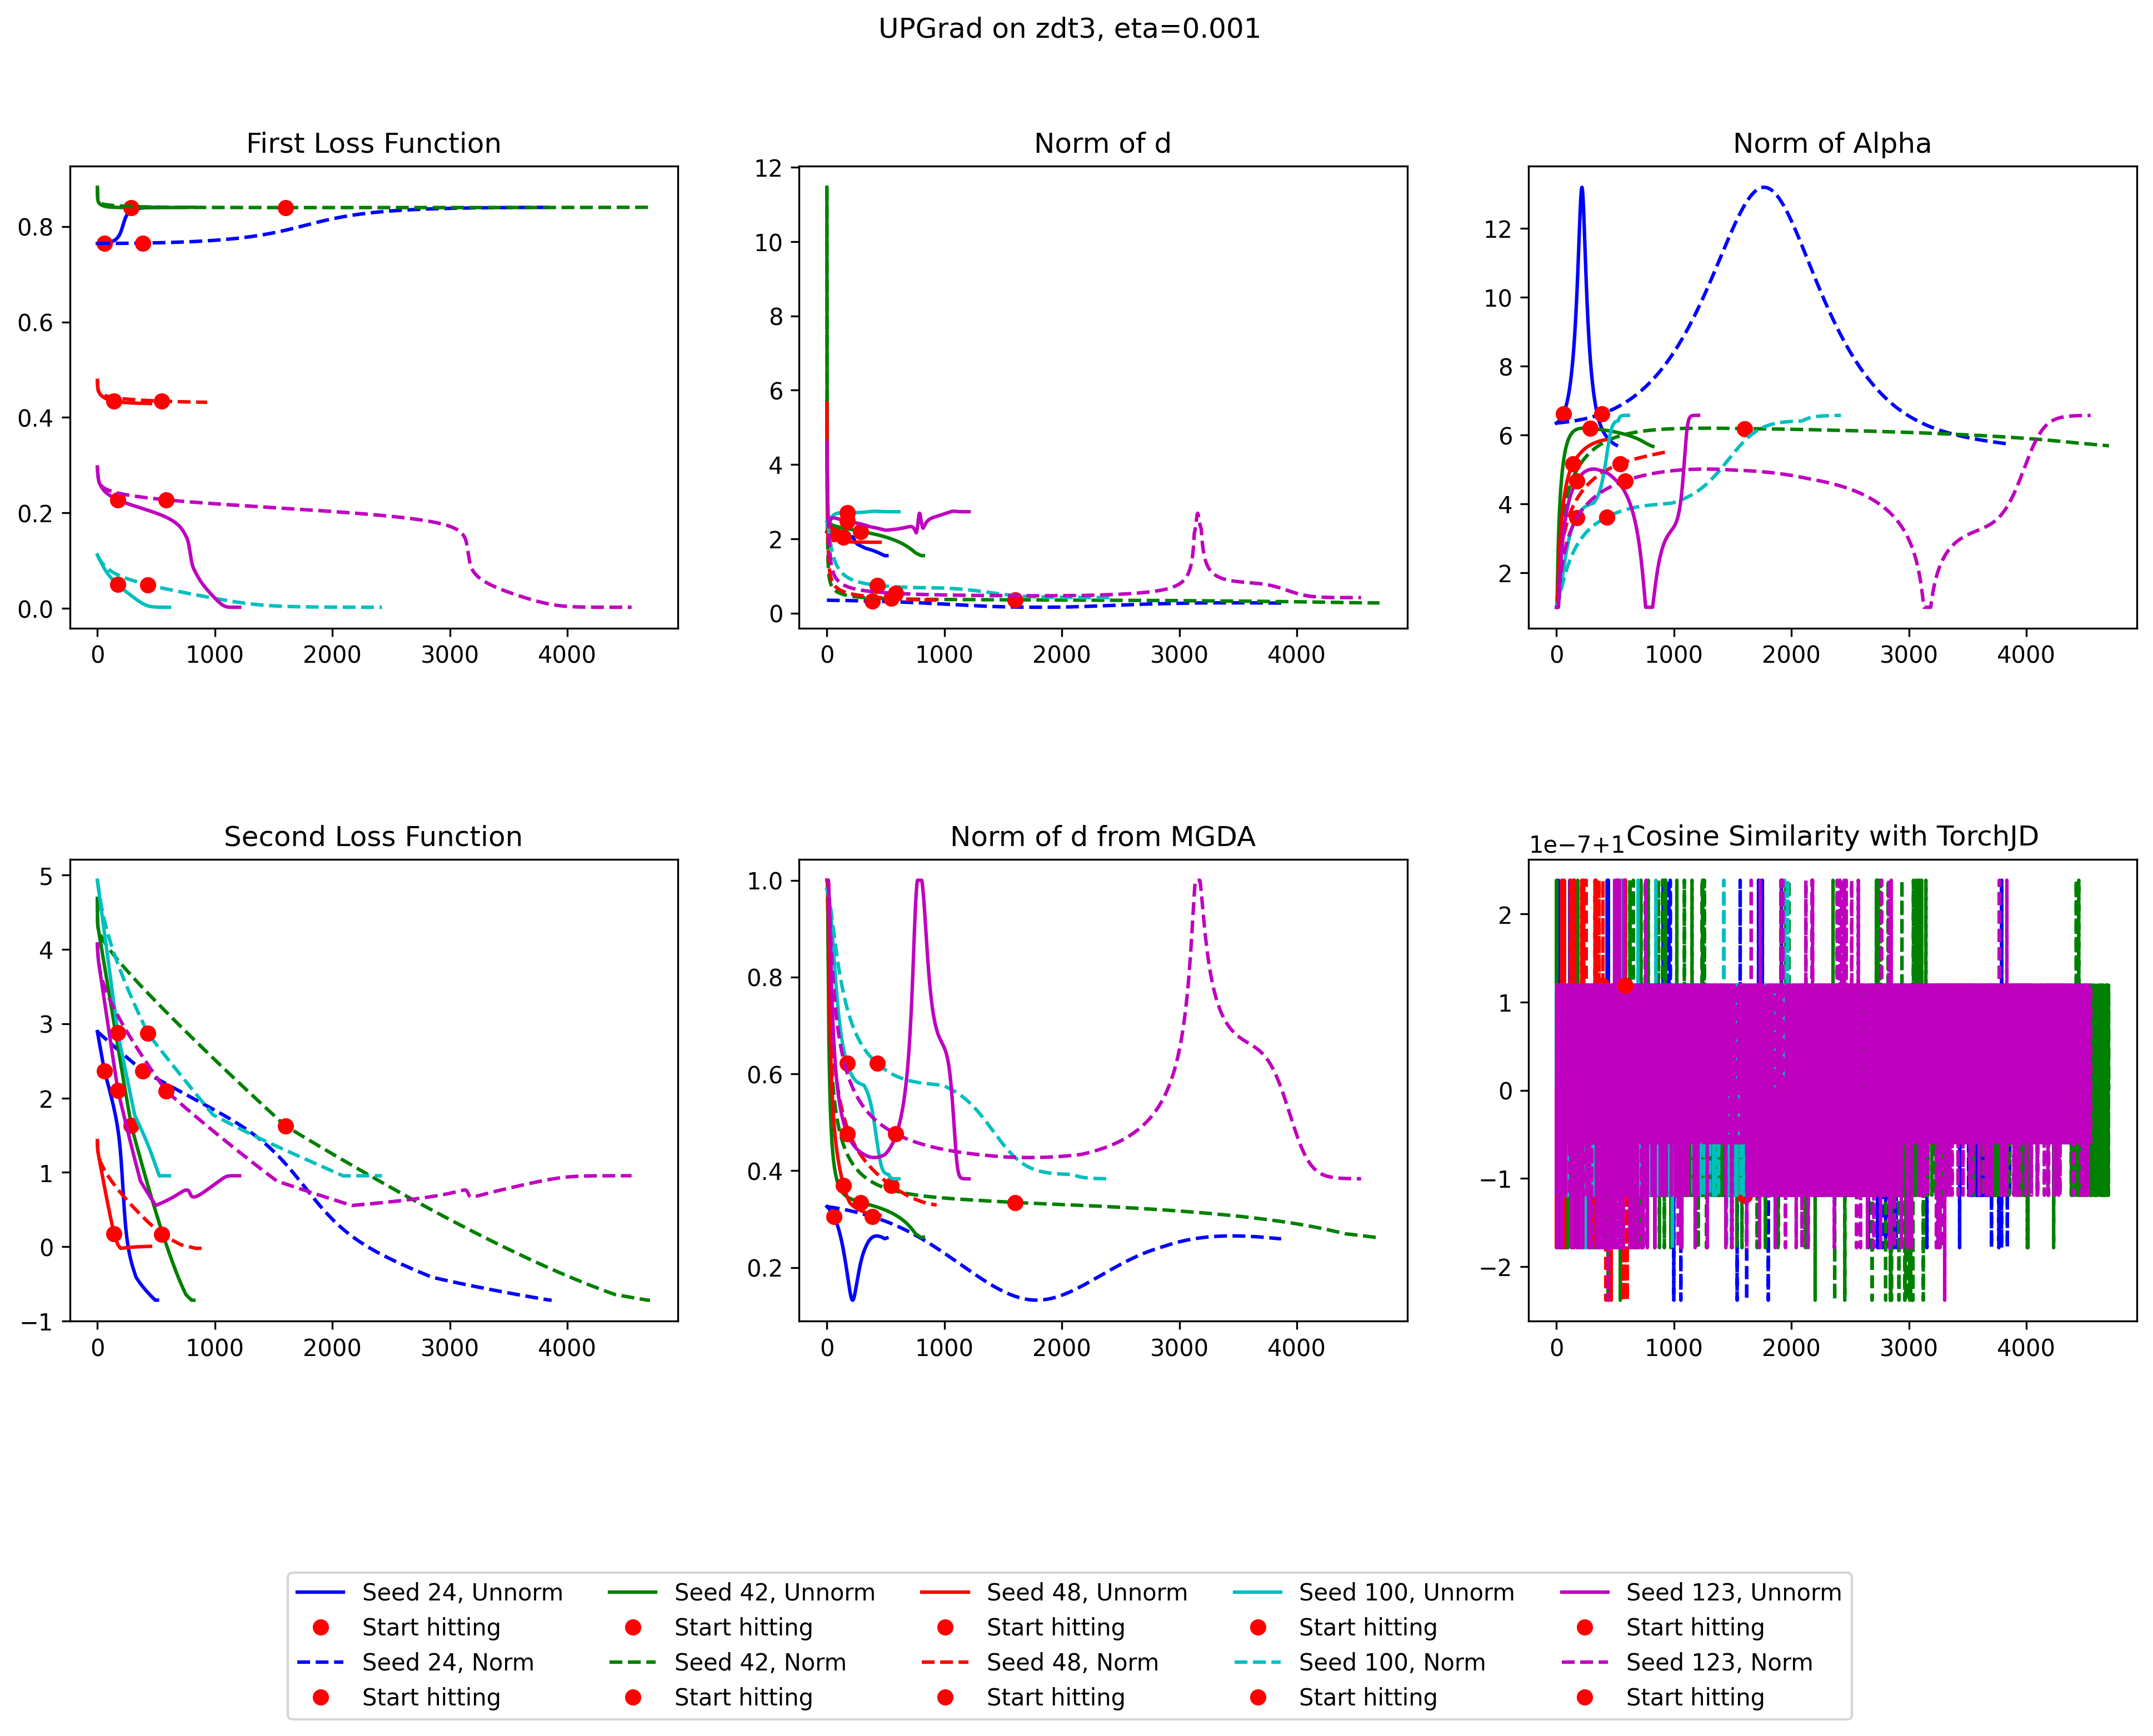
\includegraphics[scale=0.4]{UPGrad_zdt3.png}
            \caption{Testing UPGrad on ZDT3, dimension = 4, learning rate = 0.001, max iteration = 10000, seeds = 24, 42, 48, 100, 123. Red dots: $x_t$ hits boundary; green dots: $x_t$ reenters interior.}
        \end{figure}
    \end{center}
    \section{Nash-MTL}
    In , the weighting vector $\alpha$ is obtained by solving 
    \begin{equation*}
        J^TJ\alpha = \frac{1}{\alpha}, \text{ where } 1/\alpha = \mat{1/\alpha_1 & 1/\alpha_2 & \cdots & 1/\alpha_n}^T
    \end{equation*}
    But since there are no directly way to solve the equation numerically, it needs to be traslated into the minimization problem 
    \begin{equation*}
    \text{Minimise } \nabla \varphi(\alpha_{t-1})^T (\alpha_t - \alpha_{t-1}) + \sum_i \beta_i(\alpha)
    \end{equation*}
    with constraints 
    \begin{equation*}
        -\varphi_i(\alpha_t) \leq 0, \quad \alpha_t^i \geq 0,
    \end{equation*}
    To improve accuracy, we will run the quadratic solver several times, each time substituting the $\alpha$ obtained from the last iteration as $\alpha_0$.\\
    However, empirical experiment showed that the $\alpha$ reusulting from the minimization problem often mismatch the theoretical value obtained from solving $J^T J \alpha = 1/\alpha$. Quinton and Rey were quite skeptical with the official implementation, believing that it may mismatch the desired objective.
    In the official implementation of Nash-MTL, $\alpha$ is normalised with the following alogorithm.
    \begin{algorithm}[!ht]
        \caption{Nash-MTL $\alpha$ normalisation}
        \KwInput{$\alpha\in R^n, J\in R^{d\times n}, M\in \R_{>0}$}
        \Comment{$M$ is the maximum norm. It is set to $1$ by default.}
        \If{$||J^T\alpha||_2 > M$}{
            $\alpha\gets \alpha * \frac{M}{||J^T\alpha||_2}$\;
        }
        \KwOutput{$\alpha$}
    \end{algorithm}
    The normalization is not being mentioned in Navon, so it is not being included in our implementation.\\
    Nevertheless, the motivation for including the normalization can be seen from our experiment. In running Nash-MTL on all three synthetic problems, the norm of $\alpha$ can reach as high as $6000$ which in undesirable. By clipping the magnitude of $\alpha$ to the maximum norm in case $\alpha$ becomes to large, it prevents a $d$ with too large a magnitude. While the normalization method of Nash-MTL's official implementation requires manual determination of the maxmimum norm, our normalsation is more principled and without any need for manually determining a maximum norm.\\
    In agreement to previous experiments on other aggregators, employing our normalisation results in slower convergence, but also smoother curves. In solving VLMOP2, the quadratic problem is occasionally unsolvable as the minimization is unbounded. This is indicated when sharp turns occurs on the graphs. Although our normalisation cannot prevent this issue, it managed to smooth out all curve present in our plot. 
    \section{Appendix : Derivation of Nash-MTL Minimization problem}
    In the process of carrying out Nash-MTL, one needs to find the solution of
    \begin{equation*}
    G^T G \alpha = \frac{1}{\alpha},
    \end{equation*}
    where $\frac{1}{\alpha}$ represents the vector $\begin{pmatrix} \frac{1}{\alpha_1} & \frac{1}{\alpha_2} & \cdots & \frac{1}{\alpha_n} \end{pmatrix}^T$.

    To allow the computer to solve the equation, we need to turn it into a minimization problem. Taking the logarithm,
    \begin{align*}
    G^T G \alpha &= \frac{1}{\alpha} \\
    \log(\alpha_i) + \log(\beta_i(\alpha)) &= 0
    \end{align*}
    for any $i \in \{1, 2, \dots, n\}$, where $G = \begin{pmatrix} g_1 & g_2 & \cdots & g_n \end{pmatrix}$ and $\beta_i(\alpha) = g_i^T G \alpha$.

    Define $\varphi_i(\alpha) = \log(\alpha_i) + \log(\beta_i(\alpha))$ and $\varphi(\alpha) = \sum_i \varphi_i(\alpha)$. Parsing into a minimization problem, we have
    \begin{align*}
    \text{Minimize } & \varphi(\alpha) \\
    \text{with constraints } & -\varphi_i(\alpha) \leq 0, \alpha_i \geq 0
    \end{align*}
    for any $i \in \{1, 2, \dots, n\}$.

    Empirical results show that
    \begin{align*}
    \text{Minimize } & \varphi(\alpha) + \sum_i \beta_i(\alpha) \\
    \text{with constraints } & -\varphi_i(\alpha) \leq 0, \alpha_i \geq 0
    \end{align*}
    yields better results. However, the objective function is no longer convex. Hence, we approximate $\varphi_i$ with the second-order Taylor polynomial
    \begin{equation*}
    \tilde{\varphi}(\alpha_t) = \varphi(\alpha_{t-1}) + \nabla \varphi(\alpha_{t-1})(\alpha_t - \alpha_{t-1}).
    \end{equation*}
    Computing $\nabla \varphi(\alpha_{t-1})(\alpha_t - \alpha_{t-1})$, we have
    \begin{align*}
    \frac{\partial \varphi}{\partial \alpha_j} &= \frac{\partial}{\partial \alpha_j} \sum_i \log(\alpha_i) + \log(g_i^T G \alpha) \\
    &= \frac{1}{\alpha_j} + \sum_i \frac{g_i^T g_j}{g_i^T G \alpha} \\
    &= \frac{1}{\alpha_j} + \sum_i \frac{(G^T G)_{ji}}{\beta_i(\alpha)} \\
    &= \left( \frac{1}{\alpha} + G^T G \frac{1}{\beta(\alpha)} \right)_j \\
    \nabla \varphi(\alpha_{t-1})^T (\alpha_t - \alpha_{t-1}) &= \left\langle \frac{1}{\alpha_{t-1}} + G^T G \frac{1}{\beta(\alpha_{t-1})}, \alpha_t - \alpha_{t-1} \right\rangle
    \end{align*}
    Since $\varphi(\alpha_{t-1})$ is a constant, we can drop the term in the minimization problem
    \begin{align*}
    \text{Minimize } & \nabla \varphi(\alpha_{t-1})^T (\alpha_t - \alpha_{t-1}) + \sum_i \beta_i(\alpha) \\
    \text{with constraints } & -\varphi_i(\alpha_t) \leq 0, \alpha_t^i \geq 0,
    \end{align*}
    where we iterate the process several times.
\end{document}